% 2020 数值计算 报告
% c28size
% author:lyl


% ---------------------------------封面 --------------------------------- %
\documentclass[12pt]{ctexart}
\title{数值计算实验报告}
\author{李云龙}
\date{\today}



% -------------------------调用包及一些设置-------------------------------- %
\usepackage[colorlinks=true]{hyperref}
\usepackage{amsmath}
\usepackage[left=1.5cm,right=1.5cm,top=2cm,bottom=3cm]{geometry}
\usepackage{csvsimple}
\usepackage{tikz}   % 画图
\usepackage{pgfplots}
\setcounter{secnumdepth}{4}
\setcounter{tocdepth}{4}
\usepackage{listings}
\usepackage{fontspec}
\setmonofont{Consolas}
\usepackage{xcolor}
\usepackage{graphicx}
\usepackage{subfigure} 
\graphicspath{{image/}}
\usepackage[ruled]{algorithm2e}%,linesnumbered
%\usepackage{geometry}
%\geometry{a4paper,scale=0.8}
%\geometry{a4paper,left=2cm,right=2cm,top=1cm,bottom=1cm}


% ----------------------------代码显示设置-------------------------------- %
\lstset{
	rulesepcolor=\color{red!20!green!20!blue!20}, %代码块边框颜色
	breaklines=true,  %代码过长则换行
	numbers=left, %行号在左侧显示
	numberstyle=\tiny,%行号字体
	keywordstyle=\color{blue},%关键字颜色
	commentstyle=\color{gray}, %注释颜色
	frame=shadowbox, %用方框框住代码块
	basicstyle=\ttfamily,
	tabsize=4,
	xleftmargin=2em, xrightmargin=2em, aboveskip=1em, framexleftmargin=2em
}



% -----------------------------正文部分---------------------------------- %
\begin{document}
	
% --------------------------------封面----------------------------------- %
	\begin{titlepage}%\maketitle
		\newcommand{\HRule}{\rule{\linewidth}{0.5mm}}
		\centering\includegraphics[width=17cm]{logo.png}\\[1cm] 
		\centering
		\quad\\[1.5cm]
		\textsl{\Large 山东大学 }\\[0.5cm] 
		\textsl{\large 计算机科学与技术学院}\\[0.5cm] 
		\makeatletter
		\HRule \\[0.4cm]
		{ \huge \bfseries \@title}\\[0.4cm] 
		\HRule \\[1.5cm]
		\begin{minipage}{0.4\textwidth}
			\begin{flushleft} \large
				\emph{Author:}\\
				\@author 
			\end{flushleft}
		\end{minipage}
		~
		\begin{minipage}{0.4\textwidth}
			\begin{flushright} \large
				\emph{Supervisor:} \\
				\textup{刘保东}
			\end{flushright}
		\end{minipage}\\[3cm]
		\makeatother
		{\large 专业:人工智能}\\[0.5cm]
		{\large \emph{学号:201822130233}}\\[0.5cm]
		{\large \today}\\[2cm] 
		\vfill 
	\end{titlepage}
	\newpage\tableofcontents\newpage

\newpage
	\section{Summary}
	\label{sec:0}
	数值分析是研究基本数学问题的适合计算机求解的数值计算方法,包
	含了数值代数(线性方程组的解法、矩阵特征值计算等)、非线性方程求解的解法、数值逼近、数值微分和数值积分、常微分方程的数值解法等。
	它的基本理论和研究方法建立在数学理论基础之上,研究对象是数学问题,是数学的分支之一;又与计算机科学有密切的关系。我们在考虑算法时,同时要考虑计算机的特性,考虑程序设计时的可行性和复杂性。
\newpage

\newpage
% -------------------------------第1章----------------------------------- %
	\section{Chapter 1\quad 误差理论}
	\label{sec:1}
	
% ----------------------------实验题目 1.-------------------------------- %
	\subsection{实验题目 1}
	\textit{Topic description:}
	
	求方程$x^2+(\alpha+\beta)x+10^9=0$的根,其中$\alpha=-10^9$,$\beta=-1$,讨论如何设计计算格式才能有效地减少误差,提高计算精度。
	
	\textit{Answer:}
	
	设方程$ax^2+bx+c=0,a\neq0,b^2-4ac>0$。通过二次根公式可以解出方程的根
	\begin{equation}
	x_1=\frac{-b+\sqrt{b^2-4ac}}{2a},\quad x_2=\frac{-b-\sqrt{b^2-4ac}}{2a}\label{e1_1_1}
	\end{equation}
	
	等价于
	\begin{equation}
	x_1=\frac{-2c}{b+\sqrt{b^2-4ac}},\quad x_2=\frac{-2c}{b-\sqrt{b^2-4ac}}\label{e1_1_2}
	\end{equation}
	
	这种计算格式可以在$|b|\approx\sqrt{b^2-4ac}$时,避免分母过小而引起巨量消失带来的精度损失。此时,分情况讨论:
	
	(1)$b>0$时,使用(\ref{e1_1_2})计算$x_1$,使用(\ref{e1_1_1})计算$x_2$
	
	(2)$b<0$时,使用(\ref{e1_1_1})计算$x_1$,使用(\ref{e1_1_2})计算$x_2$
	
	\begin{table}[htbp]
		\centering
		\caption{第1章 第1题 最终求解结果}
		\begin{tabular}
			{c|c|c}
			\hline
			equation&$x_1$&$x_2$ \\
			\hline
			$x^2+(-1e9-1)x+1e9=0$&1e9&1 \\
			\hline
		\end{tabular}
	\end{table}

	\textit{Code:}
	
% ----------------------------------代码-------------------------------- %
	\begin{lstlisting}[language=MATLAB]
function [x1,x2] = SolveQuadraticEquations(a, b, c)
%  求解二次方程
	eps = 1e-8;
	if abs(abs(b) - sqrt(b * b - 4 * a * c)) < eps
		x1 = (-b + sqrt(b * b - 4 * a * c)) / (2 * a);
		x2 = (-b - sqrt(b * b - 4 * a * c)) / (2 * a);
	else
		if b > 0
			x1 = -2 * c / (b + sqrt(b * b - 4 * a * c));
			x2 = (-b - sqrt(b * b - 4 * a * c)) / (2 * a);
		elseif b < 0
			x1 = (-b + sqrt(b * b - 4 * a * c)) / (2 * a);
			x2 = -2 * c / (b - sqrt(b * b - 4 * a * c));
		else
			x1 = sqrt(-c / a);
			x2 = sqrt(-c / a);
		end
	end
end
	\end{lstlisting}	
	
	调用$SolveQuadraticEquations$函数,得到解$x_1$和$x_2$

% ----------------------------------代码-------------------------------- %
	\begin{lstlisting}[language=MATLAB]
% 第1章实验第1题
a = 1; alpha = -1e9; beta = -1; c = 1e9;
[x1, x2] = SolveQuadraticEquations(a, alpha + beta, c);
	\end{lstlisting}
	
% ----------------------------实验题目 2.------------------------------ %
	\subsection{实验题目 2}
	\textit{Topic description:}
	
	以计算$x^{31}$为例,讨论如何设计计算格式才能减少计算次数。

	\textit{Answer:}
	
	累乘需要$31-1=30$次乘法运算,使用快速幂算法可以减少计算次数
	
	$x^{31}=x^{16}*x^{8}*x^{4}*x^{2}*x$需要$5+4=9$次运算
	
	复杂度由$O(n)$降到了$O(\log_2 n)$
	
	\textit{Code:}
	
% ----------------------------------代码-------------------------------- %
	\begin{lstlisting}[language = C++]
// C++快速幂函数模板
long long qpow(long long a, long long b, long long mod) {
	long long ans = 1;
	while(b) {
		if(b & 1) ans = ans * a % mod;
		a = a * a % mod;
		b >>= 1;
	}
	return ans;
}
	\end{lstlisting}
\newpage


\newpage
% --------------------------------第2章-------------------------------- %
	\section{Chapter 2\quad 非线性方程求根}
	\label{sec:2}
	
% ----------------------------实验题目 1.-------------------------------- %
	\subsection{实验题目 1}
	\textit{Topic description:}
	
	求方程$2x^2+x-15=0$的正根($x^*=2.5$)近似值,分别利用如下三种格式编程计算:
	
	1.$x_{k+1}=15-x_k^2,k=0,1,2,\cdots$,取初始值$x_0=2$.
	
	2.$x_{k+1}=\frac{15}{2x_k+1},k=0,1,2,\cdots$,取初始值$x_0=2$.
	
	3.$x_{k+1}=x_k-\frac{2x_k^2+x_k-15}{4x_k+1},k=0,1,2,\cdots$,取初始值$x_0=2$.
	
	依次计算$x_1,x_2,\cdots,x_k,\cdots$,并作图观察解的稳定性,收敛性,并分析其原因。
	
	\textit{Answer:}
	
	\textbf{求根问题和求不动点问题}在下面的意义下是等价的:
	
	给定一个求根问题$f(p)=0$,可用多种方式定义具有不动点$p$的函数$g$,如$g(x)=x-
	f(x)$或$g(x)=x+3f(x)$等。相反,如果函数$g$在点$p$具有不动点,则由$f(x)=x-g(x)$所定义的函数具有零点$p$。
	
	\textbf{不动点的存在性和唯一性的充分条件}:
	
	a.如果$g\in C[a,b]$且$g(x)\in[a,b]$对一切$x\in [a,b]$成立,则$g$在$[a,b]$有一个不动点。
	
	b.除上述条件外,如果$g^{'}(x)$在$(a,b)$存在,且存在一个正常数$k<1$使得$$|g^{'}(x)|\leq k$$对一切$x\in(a,b)$成立,则不动点在$[a,b]$是唯一的。
	
	\textbf{不动点迭代}:
	
	为了求函数$g$的不动点的近似值,选择一个初始近似值$p_0$,然后通过$p_n=g(p_{n-1})(n\geq 1)$产生序列$\{p_n\}_{n-0}^{\infty}$。如果序列收敛于$p$且$g$是连续的,则$$p=\lim\limits_{n\rightarrow\infty}p_n=\lim\limits_{n\rightarrow\infty}g(p_{n-1})=g(\lim\limits_{n\rightarrow\infty}p_{n-1})=g(p)$$这样就得到了$x=g(x)$的解。
	
	\begin{figure}[htbp]
		\centering
		\subfigure[$x_{k+1}=15-x_k^2$]{
			\includegraphics[scale=0.6]{e2_1_x1.eps}
		} \quad
		\subfigure[$x_{k+1}=\frac{15}{2x_k+1}$]{
			\includegraphics[scale=0.6]{e2_1_x2.eps}
		} \quad
		\subfigure[$x_{k+1}=x_k-\frac{2x_k^2+x_k-15}{4x_k+1}$]{
			\includegraphics[scale=0.6]{e2_1_x3.eps}
		}
	\caption{第2章 第1题 实验结果}
	\end{figure}
	
	观察图(a)可知,$x_{k+1}=15-x_k^2$计算格式下不动点迭代求出的$x$发散,解趋向于无穷大,不收敛也不稳定。
	
	原因:令$g(x)=15-x^2$,则$g^{'}(x)=-2x$,取$x^*=2.5,|g^{'}(2.5)|=5>1$,因此迭代过程不收敛。
	
	观察图(b)可知,$x_{k+1}=\frac{15}{2x_k+1}$计算格式下不动点迭代求出的$x$收敛,收敛性和稳定性较好,收敛速度较慢。
	
	原因:令$g(x)=\frac{15}{2x+1}$,则$g^{'}(x)=-\frac{30}{(2x+1)^2}$,取$x^*=2.5,|g^{'}(2.5)|=\frac{5}{6}<1$,因此迭代过程收敛,收敛速率是线性的。
	
	观察图(c)可知,$x_{k+1}=x_k-\frac{2x_k^2+x_k-15}{4x_k+1}$计算格式下不动点迭代求出的$x$收敛,收敛性和稳定性好,收敛速度很快。

	原因:令$g(x)=x-\frac{2x^2+x-15}{4x+1}$,则$g^{'}(x)=1-\frac{(4x+1)^2-4(2x^2+x-15)}{(4x+1)^2}$,取$x^*=2.5,|g^{'}(2.5)|=0$,因此迭代过程收敛,收敛速率至少是二次的。
	
	这告诉我们,在不动点处导数值为零的函数是寻找二次收敛的不动点方法的函数范围。
		
	\textit{algorithm:}
	
	\begin{algorithm}
		\caption{Fixed-Point Iteration Method}
		\KwIn{initial approximation $p$; tolerance $TOL$; maximum number of iterations $N$}
		\KwOut{approximation solution $p$ or message of failure}
		Set $i=1$;
		
		\While{$i\leq N$}
		{
			Set $p=g(p_0)$;
			
			\If{$|p-p_0|<TOL$}{
				OUTPUT($p$);(Procedure completed successfully)
				
				STOP;
			}
			
			Set $i=i+1$; $p_0=p$;
		}
		
		OUTPUT("Method failed after N iterations");(Procedure completed unsuccessfully)
		
		STOP;
	\end{algorithm}
	
	\textit{Code:}
	
% ----------------------------------代码-------------------------------- %
	\begin{lstlisting}[language = MATLAB]
% 第2章第1题
iter = 45;
x1 = zeros(iter, 1); x2 = zeros(iter, 1); x3 = zeros(iter, 1);
x1(1) = 2; x2(1) = 2; x3(1) = 2;
for i = 2:iter
	x1(i) = 15 - x1(i-1)^2;
	x2(i) = 15 / (2 * x2(i-1) + 1);
	x3(i) = x3(i-1) - (2*x3(i-1)^2+x3(i-1)-15) / (4*x3(i-1)+1);
end
plot(1:iter, x1, 'r');
hold on;
plot(1:iter, x2, 'g');
hold on;
plot(1:iter, x3, 'b');
xlabel("iteration");
ylabel("x");
legend('15-x^2', '15/(2*x+1)', 'x-(2*x^2+x-15)/(4*x+1)');
	\end{lstlisting}
	
% ----------------------------实验题目 2.-------------------------------- %
	\subsection{实验题目 2}
	\textit{Topic description:}
	
	证明方程$2-3x-\sin(x)=0$在$(0,1)$内有且只有一个实根,使用二分法求误差不大于$0.0005$的根,及其需要的迭代次数。
	
	\textit{Answer:}
	
	\textbf{二分法}:
	
	假设$f$是定义在区间$[a,b]$上的连续函数,且$f(a)$和$f(b)$反号。根据介值定理,在$(a,b)$内存在一个数$p$使得$f(p)=0$。虽然当在区间$(a,b)$内存在多个根时下面的求解过程仍可行,为简单起见假设在这个区间内的根是唯一的。这个方法要求将$[a,b]$的子区间反复减半,在每一步找出含有$p$的那一半。
	
	为开始求根,设$a_1=a$和$b_1=b$,$p_1$是$[a,b]$的中点,即
	\begin{equation*}
	p_1=a_1+\frac{b_1-a_1}{2}=\frac{a_1+b_1}{2}
	\end{equation*}
	
	如果$f(p_1)=0$,则$p=p_1$,求解过程结束。如果$f(p_1)\neq0$,则$f(p_1)$或与$f(a_1)$同号或与$f(b_1)$同号。当$f(p_1)$与$f(a_1)$同号时,$p\in(p1,b1)$,让$a_2=p_1$和$b_2=b_1$。当$f(p_1)$与$f(a_1)$反号时,$p\in(a1,p1)$,让$a_2=a_1$和$b_2=p_1$。然后对区间$[a_2,b_2]$重复运用这个过程。
	
	\begin{table}[htbp]
		\centering
		\caption{第2章 第2题 实验结果}
		\begin{tabular}
			{c|c|c}
			\hline
			eqation&近似解&迭代次数 \\
			\hline
			$2-3x-\sin(x)=0$&0.5054&11 \\
			\hline
		\end{tabular}
	\end{table}
	
	\begin{figure}[htbp]
		\centering
		\includegraphics[scale=0.8]{e2_2.eps}
		\caption{第2章 第2题 二分法迭代过程}
	\end{figure}
	
	\textit{Proof:}
	
	原方程$2-3x-\sin(x)=0$,令$f(x)=2-3x-\sin(x)$
	
	当$x=0$时,$f(0)=2>0$;当$x=1$时,$f(1)=-1-\sin1=-1.8415<0$。
	
	因为$f^{'}(x)=-3-\cos(x)<0$在$(0,1)$始终成立,$f(x)$单调递减,所以$f(x)$在$(0,1)$内有且只有一个实根。
	
	\textit{algorithm:}
	
	\begin{algorithm}
		\caption{Bisection Method}
		\KwIn{endpoints $a,b$; tolerance $TOL$; maximum number of iterations $N$}
		\KwOut{approximation solution $p$ or message of failure}
		Set $k=1,FA=f(a)$;
		
		\While{$k\leq N$}
		{
			Set $p=a+(b-a)/2$; and compute $FP=f(p)$;
			
			\If{$FP=0$ or $(b-a)/2<TOL$}{
				OUTPUT($p$);(Procedure completed successfully)
				
				STOP;
			}
			
			Set $k=k+1$;
			
			\If{$FA\cdot FP>0$}{
				Set $a=p; FA=FP$;
			}
			\Else{Set $b=p$;}
		}
		
		OUTPUT("Method failed after N iterations");(Procedure completed unsuccessfully)
		
		STOP;
	\end{algorithm}
	
	\textit{Code:}

% ----------------------------------代码-------------------------------- %
\begin{lstlisting}[language = MATLAB]
function [iter,p] = Bisection(f,a,b,tol,N)
% 二分法
	iter = 1;
	fa = f(a);
	p = zeros(N, 1);
	while iter <= N
		p(iter) = a + (b - a) / 2;
		fp = f(p(iter));
		if fp == 0 || (b - a) / 2 < tol
			plot(1:iter, p(1:iter));
			xlabel("迭代次数");
			ylabel("根");
			p = p(iter);
			return;  % STOP
		end
		if fa * fp > 0
			a = p(iter);fa = fp;
		else
			b = p(iter);
		end
		iter = iter + 1;
	end
	disp("Method failed after N iterations");
end
\end{lstlisting}

	调用该函数使用二分法求解方程$2-3x-\sin(x)=0$的根
	
% ----------------------------------代码-------------------------------- %
\begin{lstlisting}[language = MATLAB]
% 第2章第2题
f = @(x)(2 - 3*x - sin(x));
a = 0; b = 1; tol = 0.0005; N = 30;
[iter, p] = Bisection(f, a, b, tol, N);
\end{lstlisting}
	
% ----------------------------实验题目 3.-------------------------------- %
	\subsection{实验题目 3}
	\textit{Topic description:}
	
	利用牛顿法求解方程$\frac{1}{2}+\frac{1}{4}x^2-x\sin x-\frac{1}{2}\cos 2x=0$分别取$x_0=\pi/2,5\pi,10\pi$,使得精度不超过$10^{-5}$。比较初值对计算结果的影响。
	
	\textit{Answer:}
	
	\textbf{Newton迭代法}是形如$p_n=g(p_{n-1})$的函数式迭代法,这里$$g(p_{n-1})=p_{n-1}-\frac{f(p_{n-1})}{f^{'}(p_{n-1})},\quad n\geq 1$$如果对某个$n$,$f^{'}(p_{n-1})=0$,则Newton迭代法不能继续下去,实际上,当$f^{'}$在$p$附近以远离零的某数为界时,Newton迭代法最有效。
	
	\begin{table}[htbp]
		\centering
		\caption{第2章 第3题 实验结果}
		\begin{tabular}
			{c|c|c}
			\hline
			$x_0$&近似解&迭代次数 \\
			\hline
			$\pi/2$&1.8955&15 \\
			\hline
			$\pi*5$&1.8955&19 \\
			\hline
			$\pi*10$&-1.8955&13052 \\
			\hline
		\end{tabular}
	\end{table}
	
	\begin{figure}[htbp]
		\centering
		\subfigure[$\pi/2$迭代过程]{
			\includegraphics[scale=0.6]{e2_3_x1.eps}
		} \quad
		\subfigure[$\pi*5$迭代过程]{
			\includegraphics[scale=0.6]{e2_3_x2.eps}
		} \quad
		\subfigure[$\pi*10$迭代过程]{
			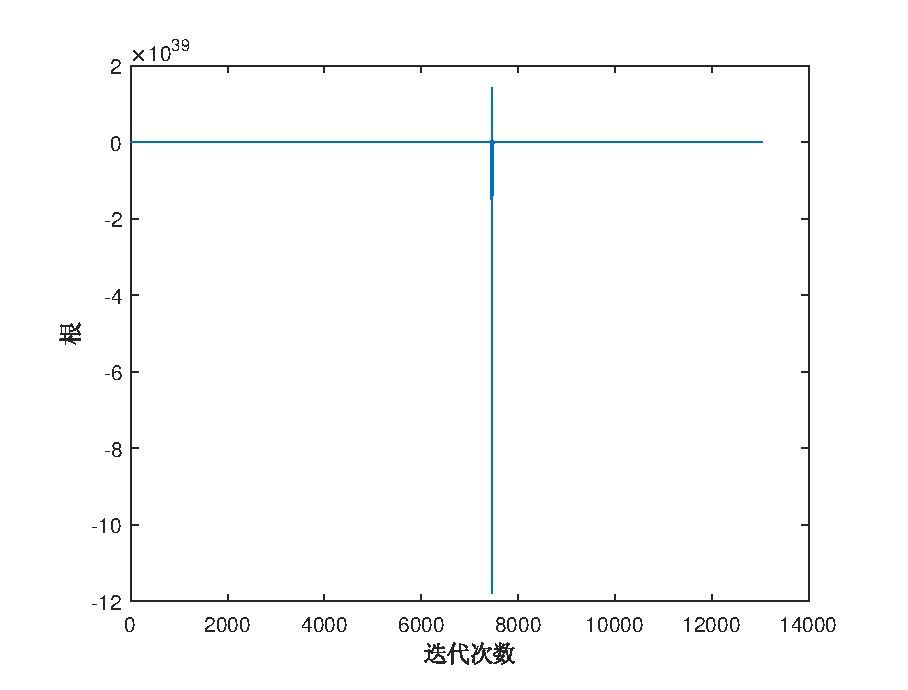
\includegraphics[scale=0.6]{e2_3_x3.eps}
		}
		\caption{$\frac{1}{2}+\frac{1}{4}x^2-x\sin x-\frac{1}{2}\cos 2x=0$取不同$x_0$收敛过程}
	\end{figure}
	
	\begin{figure}[htbp]
		\centering
		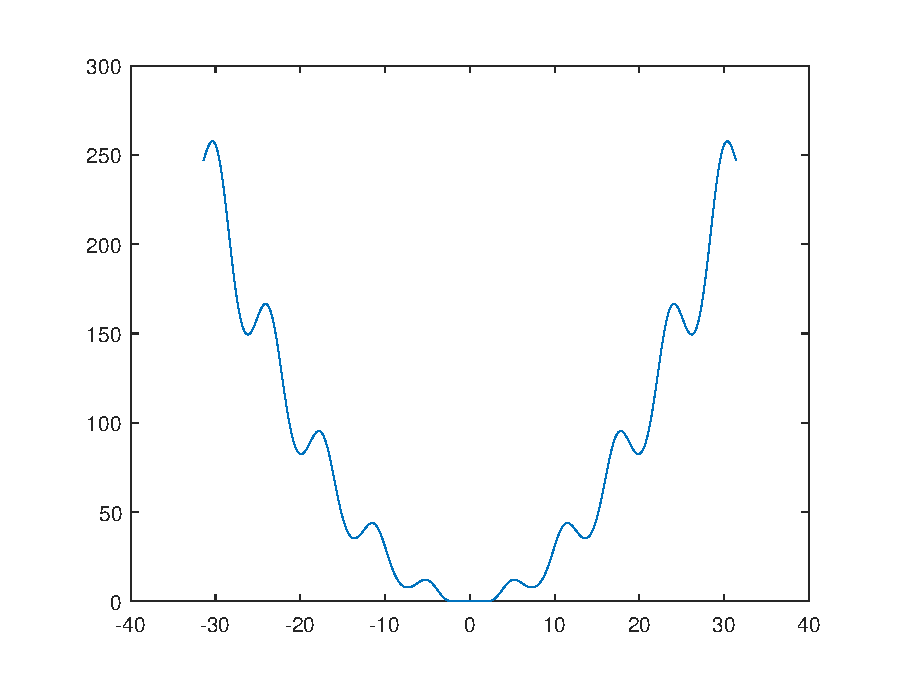
\includegraphics[scale=0.7]{e2_3_f10pi.eps}
		\caption{方程$\frac{1}{2}+\frac{1}{4}x^2-x\sin x-\frac{1}{2}\cos 2x=0$}\label{e2_3}
	\end{figure}
	
	观察图(\ref{e2_3})发现$\frac{1}{2}+\frac{1}{4}x^2-x\sin x-\frac{1}{2}\cos 2x=0$关于原点对称,取不同的初值可能会收敛到关于原点对称的不同的零点。
	
	通过实验发现,初值的选取对牛顿法的整个迭代过程和最终的解有很大影响,如果初值选取得足够好,那么算法可以在很短的迭代次数内收敛到最终解,反之如果选取的初值很坏,迭代过程中可能会有上下剧烈的起伏,迭代次数可能上万次也没法收敛。
	
	\textit{algorithm:}
	
	\begin{algorithm}
		\caption{Newton-Raphson Algorithm}
		\KwIn{initial approximation $p_0$; tolerance $TOL$; maximum number of iterations $N$}
		\KwOut{approximation solution $p$ or message of failure}
		Set $i=1$;
		
		\While{$i\leq N$}
		{
			Set $p=p_0-f(p_0)/f^{'}(p_0)$;
			
			\If{$|p-p_0|<TOL$}{
				OUTPUT($p$);(Procedure completed successfully)
				
				STOP;
			}
			
			Set $i=i+1$; $p_0=p$;
		}
		
		OUTPUT("Method failed after N iterations");(Procedure completed unsuccessfully)
		
		STOP;
	\end{algorithm}
	
	\textit{Code:}
	
% ----------------------------------代码-------------------------------- %
\begin{lstlisting}[language = MATLAB]
function [iter,x] = Newton(f,g,p0,tol,N)
% 牛顿法
	iter = 1;
	x = zeros(N, 1);
	while iter <= N
		x(iter) = p0 - f(p0) / g(p0);
		if abs(x(iter) - p0) < tol
			plot(1:iter, x(1:iter));
			xlabel("迭代次数");
			ylabel("根");
			x = x(iter);
			return;  % STOP
		end
		p0 = x(iter);
		iter = iter + 1;
	end
	disp("the method failed after N iterations");
end
\end{lstlisting}
	
	调用该函数使用牛顿法求解方程$\frac{1}{2}+\frac{1}{4}x^2-x\sin x-\frac{1}{2}\cos 2x=0$的根
	
% ----------------------------------代码-------------------------------- %
\begin{lstlisting}[language = MATLAB]
% 第2章第3题
f = @(x)(0.5 + 0.25.*x.^2 - x.*sin(x) - 0.5.*cos(2.*x));
g = @(x)(0.5.*x - sin(x) - x.*cos(x) + sin(2.*x));
p0 = [pi / 2, pi * 5, pi * 10]; tol = 1e-5; N = 14000;
[iter1, p1] = Newton(f, g, p0(1), tol, N);
[iter2, p2] = Newton(f, g, p0(2), tol, N);
[iter3, p3] = Newton(f, g, p0(3), tol, N);
\end{lstlisting}

% ---------------------------实验题目 4.------------------------------- %
	\subsection{实验题目 4}
	\textit{Topic description:}
	
	已知$f(x)=5x-e^x$在$(0,1)$之间有一个实根,试分别利用二分法、牛顿法、割线法、错位法设计相应的计算格式,并编程求解(精确到4位小数).
	
	\textit{Answer:}
	
	\textbf{正割法}:
	
	为避免Newton迭代法中求导数值的问题,引入这个方法的一个变形。由定义可知$$f^{'}(p_{n-1})=\lim\limits_{x\rightarrow p_{n-1}}\frac{f(x)-f(p_{n-1})}{x-p_{n-1}}$$让$x=p_{n-2}$,有$$f^{'}(p_{n-1})\approx \frac{f(p_{n-2})-f(p_{n-1})}{p_{n-2}-p_{n-1}}=\frac{f(p_{n-1})-f(p_{n-2})}{p_{n-1}-p_{n-2}}$$在Newton公式中用它作为$f^{'}(p_{n-1})$的近似值,得到$$p_n=p_{n-1}-\frac{f(p_{n-1})(p_{n-1}-p_{n-2})}{p_{n-1}-p_{n-2}}$$即为正割法的迭代公式。
	
	\textbf{错位法}:
	
	和正割法同样的方式产生近似解,但增加一个检验以保证在相邻的迭代之间包含根。虽然它不是通常推荐的方法,但是错位法说明了如何把根的包含整合到算法中去。
	
	\begin{figure}[htbp]
		\centering
		\subfigure[二分法迭代过程]{
			\includegraphics[scale=0.59]{e2_4_x1.eps}
		} \quad
		\subfigure[牛顿法迭代过程]{
			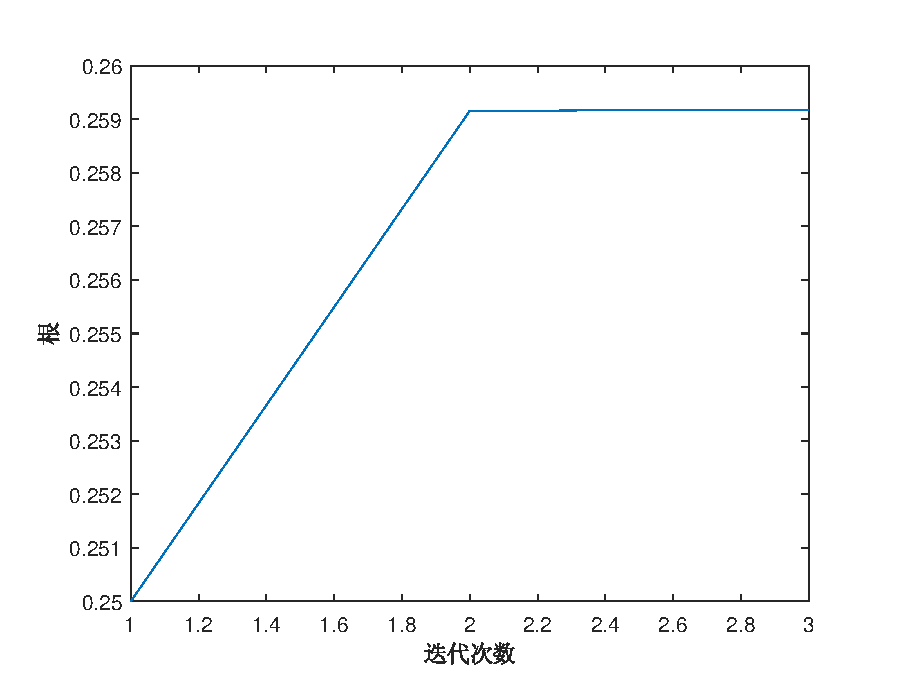
\includegraphics[scale=0.59]{e2_4_x2.eps}
		} \quad
		\subfigure[割线法迭代过程]{
			\includegraphics[scale=0.59]{e2_4_x3.eps}
		} \quad
		\subfigure[错位法迭代过程]{
			\includegraphics[scale=0.59]{e2_4_x4.eps}
		}
		\caption{第2章 第4题 $f(x)=5x-e^x$不同方法收敛过程}
	\end{figure}
	
	\begin{table}[htbp]
		\centering
		\caption{第2章 第4题 实验结果}\label{e2_4}
		\begin{tabular}
			{c|c|c}
			\hline
			计算格式&近似解&迭代次数 \\
			\hline
			二分法&0.2592&14 \\
			\hline
			牛顿法&0.2592&3 \\
			\hline
			割线法&0.2592&5 \\
			\hline
			错位法&0.2592&5 \\
			\hline
		\end{tabular}
	\end{table}
	
	通过表(\ref{e2_4})可以发现,迭代次数上牛顿法最少,二分法最多,割线法与错位法处于中间。因为二分法不要求初值,但要在整个区间内迭代,而牛顿法要求初值距离解足够近就可以快速迭代求解,割线法与错位法相当于对牛顿法做了部分修改,速度比迭代快但比牛顿法慢,并且要求初值足够靠近解才能收敛。
	
	\textit{algorithm:}
	
	\begin{algorithm}
		\caption{Secant Algorithm}
		\KwIn{initial approximation $p_0,p_1$; tolerance $TOL$; maximum number of iterations $N$}
		\KwOut{approximation solution $p$ or message of failure}
		Set $i=2; q_0=f(p_0); q_1=f(p_1);$
		
		\While{$i\leq N$}
		{
			Set $p=p_1-q_1(p_1-p_0)/(q_1-q_0)$;
			
			\If{$|p-p_0|<TOL$}{
				OUTPUT($p$);(Procedure completed successfully)
				
				STOP;
			}
			
			Set $i=i+1; p_0=p_1; q_0=q_1; p_1=p; q_1=f(p);$
		}
		
		OUTPUT("Method failed after N iterations");(Procedure completed unsuccessfully)
		
		STOP;
	\end{algorithm}

\begin{algorithm}
	\caption{False Position Algorithm}
	\KwIn{initial approximation $p_0,p_1$; tolerance $TOL$; maximum number of iterations $N$}
	\KwOut{approximation solution $p$ or message of failure}
	Set $i=2; q_0=f(p_0); q_1=f(p_1);$
	
	\While{$i\leq N$}
	{
		Set $p=p_1-q_1(p_1-p_0)/(q_1-q_0)$;
		
		\If{$|p-p_0|<TOL$}{
			OUTPUT($p$);(Procedure completed successfully)
			
			STOP;
		}
		
		Set $i=i+1; q=f(p);$
		
		\If{$q\cdot q_1<0$}{Set $p_0=p_1; q_0=q_1;$}
		
		Set $p_1=p; q_1=q;$
	}
	
	OUTPUT("Method failed after N iterations");(Procedure completed unsuccessfully)
	
	STOP;
\end{algorithm}
	
	\textit{Code:}
	
% ----------------------------------代码-------------------------------- %
二分法与牛顿法代码在上面已经给出,以下是割线法与错位法代码

\begin{lstlisting}[language = MATLAB]
function [iter,x] = Secant(f,a,b,tol,N)
% 割线法
	iter = 2;
	y0 = f(a); y1 = f(b);
	x = zeros(N, 1);
	while iter <= N
		x(iter) = b - y1 * (b - a) / (y1 - y0);
		if abs(x(iter) - b) < tol
			plot(1:iter, x(1:iter));
			xlabel("迭代次数");
			ylabel("根");
			x = x(iter);
			return;  % STOP
		end
		a = b;
		y0 = y1;
		b = x(iter);
		y1 = f(x(iter));
		iter = iter + 1;
	end
	disp("the method failed after N iterations");
end
\end{lstlisting}

\begin{lstlisting}[language = MATLAB]
function [iter,x] = FalsePosition(f,a,b,tol,N)
% 错位法
	iter = 2;
	y0 = f(a);
	y1 = f(b);
	x = zeros(N, 1);
	while iter <= N
		x(iter) = b - y1 * (b - a) / (y1 - y0);
		if abs(x(iter) - b) < tol
			plot(1:iter, x(1:iter));
			xlabel("迭代次数");
			ylabel("根");
			x = x(iter);
			return;  % STOP
		end
		y = f(x(iter));
		if y * y1 < 0
			a = b;
			y0 = y1;
		end
		b = x(iter);
		y1 = y;
		iter = iter + 1;
	end
	disp("Method failed after N iterations");
end
\end{lstlisting}
分别使用以上4种方法计算方程$5x-e^x=0$的根
\begin{lstlisting}[language = MATLAB]
% 第2章第4题
f = @(x)(5*x - exp(x));
g = @(x)(5 - exp(x));
tol = 1e-4; x0 = 0; x1 = 1; n0 = 30;
[iter1, p1] = Bisection(f, x0, x1, tol, n0);
[iter2, p2] = Newton(f, g, x0, tol, n0);
[iter3, p3] = Secant(f, x0, x1, tol, n0);
[iter4, p4] = FalsePosition(f, x0, x1, tol, n0);
\end{lstlisting}

\newpage


\newpage
% --------------------------------第3章--------------------------------- %
	\section{Chapter 3\quad 插值多项式}
	\label{sec:3}
	
% ----------------------------实验题目 1.------------------------------- %
	\subsection{实验题目 1}
	\textit{Topic description:}
	
	基于不同边界条件的样条函数计算公式推导:
	
	1.自然边界
	
	2.固定边界
	
	3.周期边界
	
	4.强制第一个子区间和第二个子区间样条多项式的三阶导数相等,倒数第二个子区间和最后一个子区间的三次样条函数的三阶导数相等
	
	\textit{Answer:}
	
	给定在区间$[a,b]$上定义的函数$f$和一组节点$a=x_0<x_1<\dots<x_n=b$,三次样条插值$S(x)$是满足下列条件的函数:
	
	a.\quad$S(x)$在子区间$x_j,x_{j+1}$\quad$(j=0,1,\dots,n-1)$上是三次多项式,记为$S_j(x)$
	
	b.\quad$S(x_j)=f(x_j)\quad(j=0,1,\dots,n)$
	
	c.\quad$S_{j+1}(x_{j+1})=S_j(x_{j+1}))\quad(j=0,1,\dots,n-2)$
	
	d.\quad$S_{j+1}^{'}(x_{j+1})=S_j^{'}(x_{j+1}))\quad(j=0,1,\dots,n-2)$
	
	e.\quad$S_{j+1}^{''}(x_{j+1})=S_j^{''}(x_{j+1}))\quad(j=0,1,\dots,n-2)$
	
	f.\quad 满足以下边界条件之一:
	
	\qquad(1)自然边界:$S^{''}(x_0)=S^{''}(x_n)=0$
	
	\qquad(2)固定边界:$S^{'}(x_0)=f^{'}(x_0),S^{'}(x_n)=f^{'}(x_n)$
	
	\qquad(3)周期边界:$S^{k}(x_0+0)=S^{k}(x_n-0)\quad (k=0,1,2)$
	
	\qquad(4)强制第一个子区间和第二个子区间样条多项式的三阶导数相等,倒数第二个子区间和最后一个子区间的三次样条函数的三阶导数相等:$S_0^{'''}(x_0)=S_1^{'''}(x_1),S_{n-2}^{'''}(x_{n-1})=S_{n-1}^{'''}(x_{n})$
	
	为了构造给定函数$f$的三次样条插值,令三次多项式
	\begin{equation*}
	S_j(x)=a_j+b_j(x-x_j)+c_j(x-x_j)^2+d_j(x-x_j)^3\quad x\in[x_j,x_{j+1}]\quad(j=0,1,\dots,n-1)
	\end{equation*}
	
	接下来的问题是如何确定参数$a_j,b_j,c_j,d_j,j=0,1,\dots,n-1$的值
	
	根据条件(b)
	\begin{equation*}
	S_j(x_j)=a_j=f(x_j),j=0,1,\dots,n
	\end{equation*}
	
	根据条件(c)
	\begin{equation*}
	a_{j+1}=S_{j+1}(x_{j+1})=S_j(x_{j+1})=a_j+b_j(x_{j+1}-x_j)+c_j(x_{j+1}-x_j)^2+d_j(x_{j+1}-x_j)^3,j=0,1,\dots,n-2
	\end{equation*}
	
	令$h_j=x_{j+1}-x_j,j=0,1,\dots,n-1$且有$a_n=f(x_n)$,则上式可写为
	\begin{equation}
	a_{j+1}=a_j+b_jh_j+c_jh_j^2+d_jh_j^3,j=0,1,\dots,n-1\label{eq:a}
	\end{equation}
	
	类似地,定义$b_n=S^{'}(x_n)$并根据条件(d)得
	\begin{equation}
	b_{j+1}=b_j+2c_jh_j+3d_jh_j^2,j=0,1,\dots,n-1\label{eq:b}
	\end{equation}
	
	定义$c_n=S^{''}(x_n)/2$并根据条件(e)得
	\begin{equation}
	c_{j+1}=c_j+3d_jh_j,j=0,1,\dots,n-1\label{eq:c}
	\end{equation}
	
	通过式(\ref{eq:c})求解$d_j$,并回代式(\ref{eq:a})和式(\ref{eq:b}),可得
	\begin{equation}
	a_{j+1}=a_j+b_jh_j+\frac{h_j^2}{3}(2c_j+c_{j+1}),j=0,1,\dots,n-1\label{eq:na}
	\end{equation}
	\begin{equation}
	b_{j+1}=b_j+h_j(c_j+c_{j+1}),j=0,1,\dots,n-1\label{eq:nb}
	\end{equation}
	
	通过式(\ref{eq:na})解出
	\begin{equation}
	b_j=\frac{1}{h_j}(a_{j+1}-a_j)-\frac{h_j}{3}(2c_j+c_{j+1}),j=0,1,\dots,n-1\label{eq:nnb}
	\end{equation}
	
	利用上式得出$b_{j-1}$表达式并待入式(\ref{eq:nb})得
	\begin{equation}
	h_{j-1}c_{j-1}+2(h_{j-1}+h_j)c_j+h_jc_{j+1}=\frac{3}{h_j}(a_{j+1}-a_j)-\frac{3}{h_{j-1}}(a_j-a_{j-1})\label{linear system}
	\end{equation}
	
	对$j=1,2,\dots,n-1$成立,因为$\{h_j\}_{j=0}^n$和$\{a_j\}_{j=0}^n$已知,该方程组中未知的值仅有$\{c_j\}_{j=0}^n$,只要确定了$\{c_j\}_{j=0}^n$的值,$\{b_j\}_{j=0}^n$和$\{d_j\}_{j=0}^n$可以很轻松地从式(\ref{eq:nnb})和式(\ref{eq:c})中求出,从而构建出三次多项式$\{S_j(x)\}_{j=0}^{n-1}$。
	
	当施加了以上4种不同的边界条件时,就能得出$\{c_j\}_{j=0}^n$。
	
	(1)\textbf{自然边界}:
	
	如果$f$定义在$a=x_0<x_1<\dots<x_n=b$,则$f$在节点$x_0,x_1,\dots,x_n$上具有唯一的自然样条插值$S$,也就是满足边界条件$S^{''}(a)=0$和$S^{''}(b)=0$的样条插值。
	
	证明:
	
	边界条件为$c_n=S^{''}(x_n)=0$和$0=S^{''}(x_0)=2c_0+6d_0(x_0-x_0)$,因此$c_0=0$。这2个等式与式(\ref{linear system})一起可得到线性方程组$\mathbf{Ax}=\mathbf{b}$,其中$\mathbf{A}$是$(n+1)\times(n+1)$矩阵
	
	\[
	\mathbf{A}=\begin{bmatrix}
	1&0&0&\dots&\dots&0 \\
	h_0&2(h_0+h_1)&h_1&\ddots&\ddots&\vdots \\
	0&h_1&2(h_1+h_2)&\ddots&\ddots&\vdots \\
	\vdots&\ddots&\ddots&\ddots&\ddots&0 \\
	\vdots&\ddots&\ddots&h_{n-2}&2(h_{n-2}+h_{n-1})&h_{n-1} \\
	0&\dots&\dots&0&0&1
	\end{bmatrix}
	\]
	
	\[
	\mathbf{b}=\begin{bmatrix}
	0 \\
	\frac{3}{h_1}(a_2-a_1)-\frac{3}{h_0}(a_1-a_0) \\
	\vdots \\
	\frac{3}{h_{n-1}}(a_n-a_{n-1})-\frac{3}{h_{n-2}}(a_{n-1}-a_{n-2}) \\
	0
	\end{bmatrix},\quad
	\mathbf{x}=\begin{bmatrix}
	c_0 \\
	c_1 \\
	c_2 \\
	\vdots \\
	c_n
	\end{bmatrix}
	\]
	
	矩阵$\mathbf{A}$为严格对角占优矩阵,从而线性方程组对于$c_0,c_1,\dots,c_n$有唯一解。
	
	(2)\textbf{固定边界}:
	
	如果$f$定义在$a=x_0<x_1<\dots<x_n=b$并且在$a$和$b$点上可微,则$f$在节点$x_0,x_1,\dots,x_n$上具有唯一的固定样条插值$S$,也就是满足边界条件$S^{'}(a)=f^{'}(a)$和$S^{'}(b)=f^{'}(b)$的样条插值。
	
	证明:
	
	因为$S^{'}(a)=f^{'}(a)=S^{'}(x_0)=b_0$,根据式(\ref{eq:nnb})取$j=0$得
	
	\begin{equation*}
	S^{'}(a)=S^{'}(x_0)=b_0=\frac{a_1-a_0}{h_0}-\frac{h_0(2c_0+c_1)}{3}=f^{'}(a)
	\end{equation*}
	\begin{equation*}
	\Rightarrow
	2h_0c_0+h_0c_1=\frac{3}{h_0}(a_1-a_0)-3f^{'}(a)
	\end{equation*}
	
	同理,因为$S^{'}(b)=f^{'}(b)$,根据式(\ref{eq:nb})和式(\ref{eq:nnb})取$j=n-1$得
	\begin{equation*}
	\begin{split}
	f^{'}(b)=b_n&=b_{n-1}+h_{n-1}(c_{n-1}+c_n) \\
	&=\frac{a_n-a_{n-1}}{h_{n-1}}-\frac{h_{n-1}}{3}(2c_{n-1}+c_n)+h_{n-1}(c_{n-1}+c_n) \\
	&=\frac{a_n-a_{n-1}}{h_{n-1}}+\frac{h_{n-1}}{3}(c_{n-1}+2c_n)
	\end{split}
	\end{equation*}
	\begin{equation*}
	\Rightarrow
	h_{n-1}c_{n-1}+2h_{n-1}c_n=3f^{'}(b)-\frac{3}{h_{n-1}}(a_n-a_{n-1})
	\end{equation*}
	这2个等式与式(\ref{linear system})一起可得到线性方程组$\mathbf{Ax}=\mathbf{b}$,其中$\mathbf{A}$是$(n+1)\times(n+1)$矩阵
	
	\[
	\mathbf{A}=\begin{bmatrix}
	2h_0&h_0&0&\dots&\dots&0 \\
	h_0&2(h_0+h_1)&h_1&\ddots&\ddots&\vdots \\
	0&h_1&2(h_1+h_2)&\ddots&\ddots&\vdots \\
	\vdots&\ddots&\ddots&\ddots&\ddots&0 \\
	\vdots&\ddots&\ddots&h_{n-2}&2(h_{n-2}+h_{n-1})&h_{n-1} \\
	0&\dots&\dots&0&h_{n-1}&2h_{n-1}
	\end{bmatrix}
	\]
	
	\[
	\mathbf{b}=\begin{bmatrix}
	\frac{3}{h_0}(a_1-a_0)-3f^{'}(a) \\
	\frac{3}{h_1}(a_2-a_1)-\frac{3}{h_0}(a_1-a_0) \\
	\vdots \\
	\frac{3}{h_{n-1}}(a_n-a_{n-1})-\frac{3}{h_{n-2}}(a_{n-1}-a_{n-2}) \\
	3f^{'}(b)-\frac{3}{h_{n-1}}(a_n-a_{n-1})
	\end{bmatrix},\quad
	\mathbf{x}=\begin{bmatrix}
	c_0 \\
	c_1 \\
	c_2 \\
	\vdots \\
	c_n
	\end{bmatrix}
	\]
	
	矩阵$\mathbf{A}$为严格对角占优矩阵,从而线性方程组对于$c_0,c_1,\dots,c_n$有唯一解。
	
	(3)\textbf{周期边界}:
	
	如果$f$定义在$a=x_0<x_1<\dots<x_n=b$,则$f$在节点$x_0,x_1,\dots,x_n$上具有唯一的周期样条插值$S$,也就是满足边界条件$S^{k}(x_0+0)=S^{k}(x_n-0)\quad (k=0,1,2)$的样条插值。
	
	证明:
	
	因为$S^{'}(x_0+0)=S^{'}(a)=b_0=b_n=S^{'}(b)=S^{'}(x_n-0)$,根据式(\ref{eq:nnb})取$j=0$得
	
	\begin{equation*}
	b_0=\frac{a_1-a_0}{h_0}-\frac{h_0}{3}(2c_0+c_1)
	\end{equation*}
	
	再根据式(\ref{eq:nb})取$j=n-1$得
	\begin{equation*}
	\begin{split}
	b_n&=b_{n-1}+h_{n-1}(c_{n-1}+c_n) \\
	&=\frac{a_n-a_{n-1}}{h_{n-1}}-\frac{h_{n-1}}{3}(2c_{n-1}+c_n)+h_{n-1}(c_{n-1}+c_n) \\
	&=\frac{a_n-a_{n-1}}{h_{n-1}}+\frac{h_{n-1}}{3}c_{n-1}+\frac{2h_{n-1}}{3}c_n
	\end{split}
	\end{equation*}
	两式相等得
	\begin{equation*}
	\frac{2h_0}{3}c_0+\frac{h_0}{3}c_1+\frac{h_{n-1}}{3}c_{n-1}+\frac{2h_{n-1}}{3}c_n=\frac{a_1-a_0}{h_0}-\frac{a_n-a_{n-1}}{h_{n-1}}
	\end{equation*}
	
	因为$S^{''}(x_0+0)=S^{''}(a)=2c_0=2c_n=S^{''}(b)=S^{''}(x_n-0)$得
	\begin{equation*}
	c_0-c_n=0
	\end{equation*}
	
	这2个等式与式(\ref{linear system})一起可得到线性方程组$\mathbf{Ax}=\mathbf{b}$,其中$\mathbf{A}$是$(n+1)\times(n+1)$矩阵
	
	\[
	\mathbf{A}=\begin{bmatrix}
	\frac{2h_0}{3}&\frac{h_1}{3}&0&\dots&\frac{h_n}{3}&\frac{2h_n}{3} \\
	h_0&2(h_0+h_1)&h_1&\ddots&\ddots&\vdots \\
	0&h_1&2(h_1+h_2)&\ddots&\ddots&\vdots \\
	\vdots&\ddots&\ddots&\ddots&\ddots&0 \\
	\vdots&\ddots&\ddots&h_{n-2}&2(h_{n-2}+h_{n-1})&h_{n-1} \\
	1&\dots&\dots&0&0&-1
	\end{bmatrix}
	\]
	
	\[
	\mathbf{b}=\begin{bmatrix}
	\frac{a_1-a_0}{h_0}-\frac{a_n-a_{n-1}}{h_{n-1}} \\
	\frac{3}{h_1}(a_2-a_1)-\frac{3}{h_0}(a_1-a_0) \\
	\vdots \\
	\frac{3}{h_{n-1}}(a_n-a_{n-1})-\frac{3}{h_{n-2}}(a_{n-1}-a_{n-2}) \\
	0
	\end{bmatrix},\quad
	\mathbf{x}=\begin{bmatrix}
	c_0 \\
	c_1 \\
	c_2 \\
	\vdots \\
	c_n
	\end{bmatrix}
	\]
	
	线性方程组对于$c_0,c_1,\dots,c_n$有唯一解。
	
	(4)\textbf{非扭曲边界}(强制第一个子区间和第二个子区间样条多项式的三阶导数相等,倒数第二个子区间和最后一个子区间的三次样条函数的三阶导数相等):
	
	如果$f$定义在$a=x_0<x_1<\dots<x_n=b$,则$f$在节点$x_0,x_1,\dots,x_n$上具有唯一的非扭结样条插值$S$,也就是满足边界条件$S_0^{'''}(x_0)=S_1^{'''}(x_1),S_{n-2}^{'''}(x_{n-1})=S_{n-1}^{'''}(x_{n})$的样条插值。
	
	证明:
	
	因为$S_0^{'''}(x_0)=6d_0=6d_1=S_1^{'''}(x_1)$,根据式(\ref{eq:c})分别取$j=0$和$j=1$得
	
	\begin{equation*}
	d_0=\frac{c_1-c_0}{3h_0}=\frac{c_2-c_1}{3h_1}=d_1
	\end{equation*}
	\begin{equation*}
	\Rightarrow
	h_1c_0-(h_0+h_1)c_1+h_0c_2=0
	\end{equation*}
	
	同理,因为$S_{n-2}^{'''}(x_{n-1})=6d_{n-2}=6d_{n-1}=S_{n-1}^{'''}(x_n)$,根据式(\ref{eq:c})分别取$j=n-2$和$j=n-1$得
	\begin{equation*}
	d_{n-2}=\frac{c_{n-1}-c_{n-2}}{3h_{n-2}}=\frac{c_n-c_{n-1}}{3h_{n-1}}=d_{n-1}
	\end{equation*}
	\begin{equation*}
	\Rightarrow
	h_{n-1}c_{n-2}-(h_{n-2}+h_{n-1})c_{n-1}+h_{n-2}c_n=0
	\end{equation*}
	这2个等式与式(\ref{linear system})一起可得到线性方程组$\mathbf{Ax}=\mathbf{b}$,其中$\mathbf{A}$是$(n+1)\times(n+1)$矩阵
	
	\[
	\mathbf{A}=\begin{bmatrix}
	h_1&-(h_0+h_1)&h_0&\dots&\dots&0 \\
	h_0&2(h_0+h_1)&h_1&\ddots&\ddots&\vdots \\
	0&h_1&2(h_1+h_2)&\ddots&\ddots&\vdots \\
	\vdots&\ddots&\ddots&\ddots&\ddots&0 \\
	\vdots&\ddots&\ddots&h_{n-2}&2(h_{n-2}+h_{n-1})&h_{n-1} \\
	0&\dots&\dots&h_{n-1}&-(h_{n-2}+h_{n-1})&h_{n-2}
	\end{bmatrix}
	\]
	
	\[
	\mathbf{b}=\begin{bmatrix}
	0 \\
	\frac{3}{h_1}(a_2-a_1)-\frac{3}{h_0}(a_1-a_0) \\
	\vdots \\
	\frac{3}{h_{n-1}}(a_n-a_{n-1})-\frac{3}{h_{n-2}}(a_{n-1}-a_{n-2}) \\
	0
	\end{bmatrix},\quad
	\mathbf{x}=\begin{bmatrix}
	c_0 \\
	c_1 \\
	c_2 \\
	\vdots \\
	c_n
	\end{bmatrix}
	\]
	
	线性方程组对于$c_0,c_1,\dots,c_n$有唯一解。
	
% ----------------------------实验题目 2.-------------------------------- %
	\subsection{实验题目 2}
	\textit{Topic description:}
	
	以$y=sin(x)$为例,在$[0,m]$区间内生成$11$个、$21$个数据点,设计算法或程序,用上述4个边界条件,分别计算其样条插值,并作图比较,分析其差异性.
	
	\textit{Answer:}
	
	\begin{figure}[htbp]
	\centering
	\subfigure[11个数据点]{
		\includegraphics[scale=0.59]{e3_2_111.eps}
	} \quad
	\subfigure[21个数据点]{
		\includegraphics[scale=0.59]{e3_2_121.eps}
	}
	\caption{第3章 第2题 自然边界条件}
	\end{figure}

	\begin{figure}[htbp]
		\centering
		\subfigure[11个数据点及原曲线对比]{
			\includegraphics[scale=0.59]{e3_2_112.eps}
		} \quad
		\subfigure[21个数据点及原曲线对比]{
			\includegraphics[scale=0.59]{e3_2_122.eps}
		}
		\caption{第3章 第2题 自然边界条件及原曲线对比}
	\end{figure}

	\begin{figure}[htbp]
		\centering
		\subfigure[11个数据点]{
			\includegraphics[scale=0.59]{e3_2_211.eps}
		} \quad
		\subfigure[21个数据点]{
			\includegraphics[scale=0.59]{e3_2_221.eps}
		}
		\caption{第3章 第2题 固定边界条件}
	\end{figure}
	
	\begin{figure}[htbp]
		\centering
		\subfigure[11个数据点及原曲线对比]{
			\includegraphics[scale=0.59]{e3_2_212.eps}
		} \quad
		\subfigure[21个数据点及原曲线对比]{
			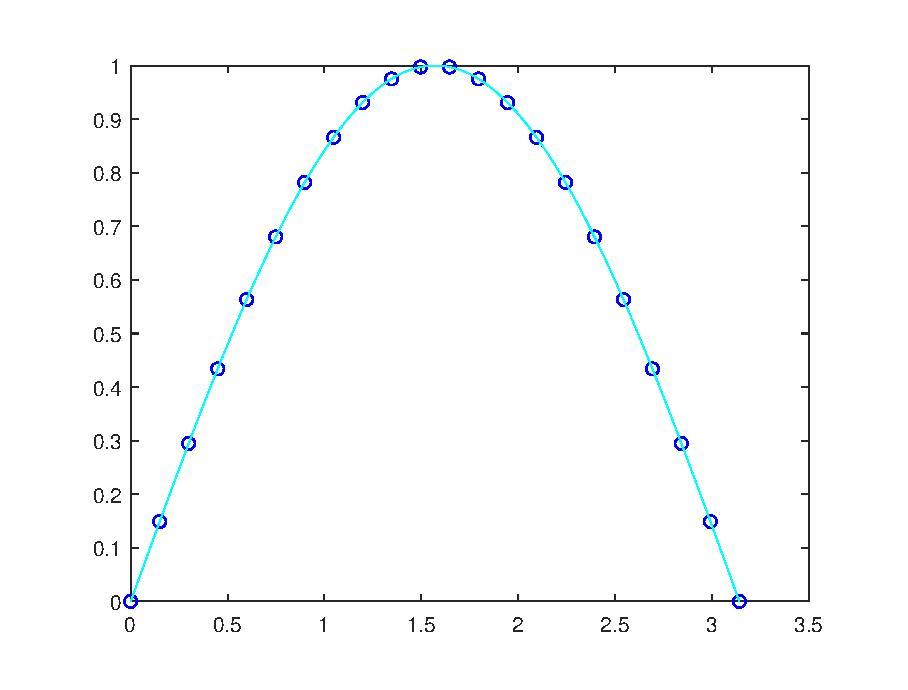
\includegraphics[scale=0.59]{e3_2_222.eps}
		}
		\caption{第3章 第2题 固定边界条件及原曲线对比}
	\end{figure}
	
	\begin{figure}[htbp]
		\centering
		\subfigure[11个数据点]{
			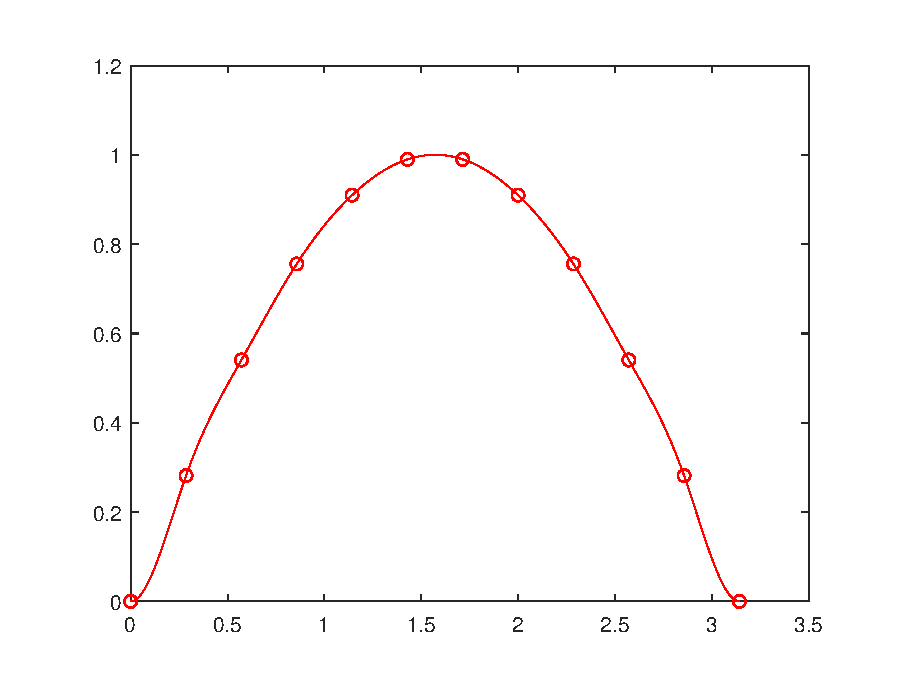
\includegraphics[scale=0.59]{e3_2_311.eps}
		} \quad
		\subfigure[21个数据点]{
			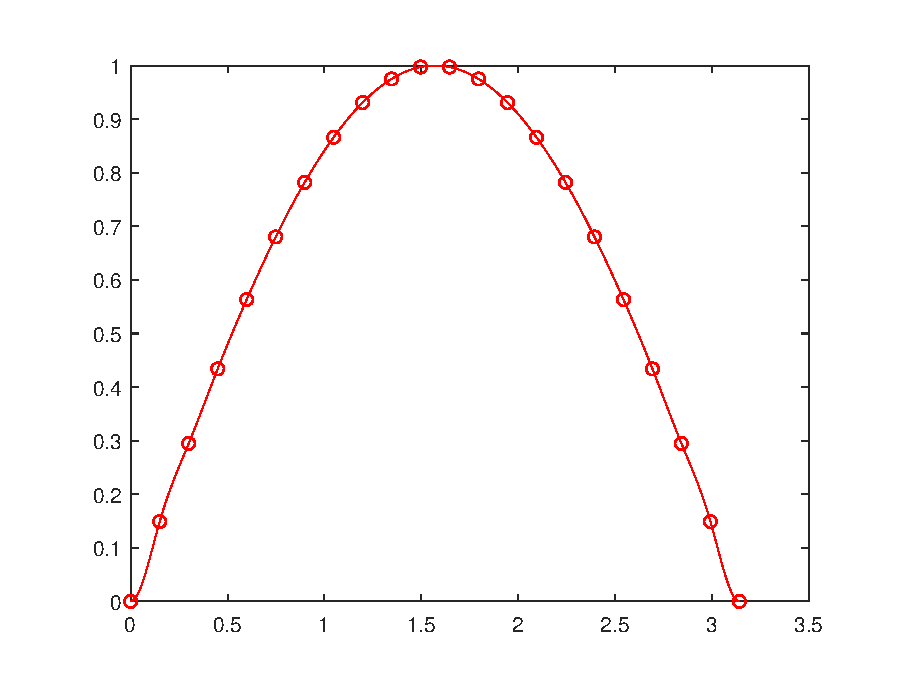
\includegraphics[scale=0.59]{e3_2_321.eps}
		}
		\caption{第3章 第2题 周期边界条件}
	\end{figure}

	\begin{figure}[htbp]
		\centering
		\subfigure[11个数据点及原曲线对比]{
			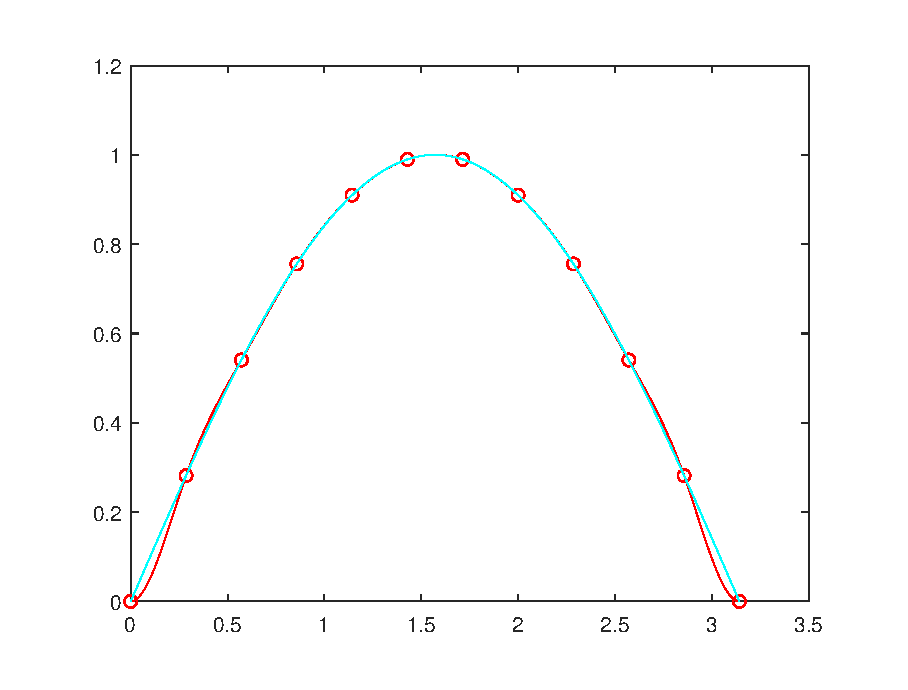
\includegraphics[scale=0.59]{e3_2_312.eps}
		} \quad
		\subfigure[21个数据点及原曲线对比]{
			\includegraphics[scale=0.59]{e3_2_322.eps}
		}
		\caption{第3章 第2题 周期边界条件及原曲线对比}
	\end{figure}
	
	\begin{figure}[htbp]
		\centering
		\subfigure[11个数据点]{
			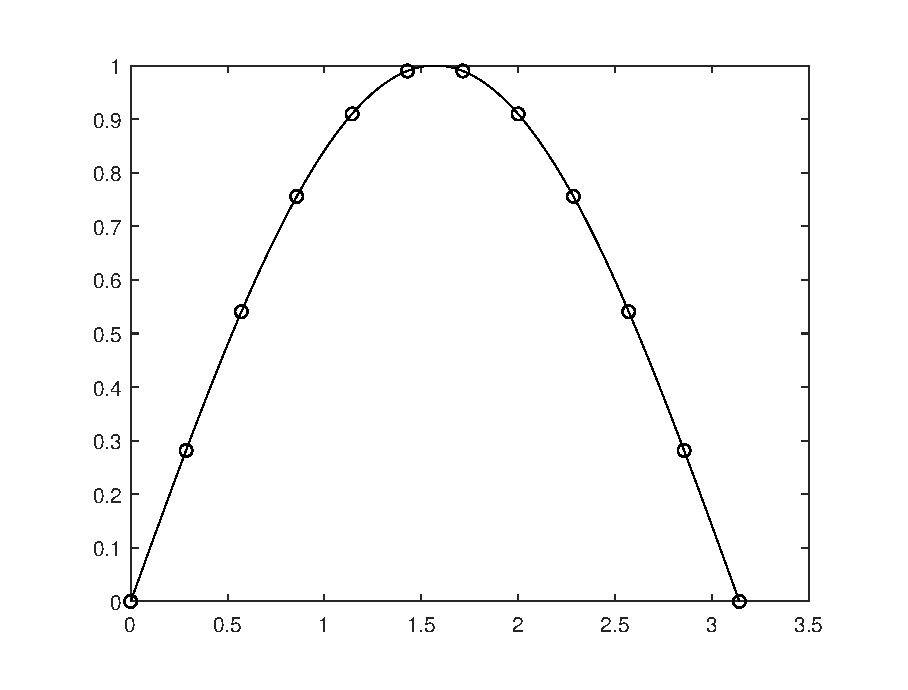
\includegraphics[scale=0.59]{e3_2_411.eps}
		} \quad
		\subfigure[21个数据点]{
			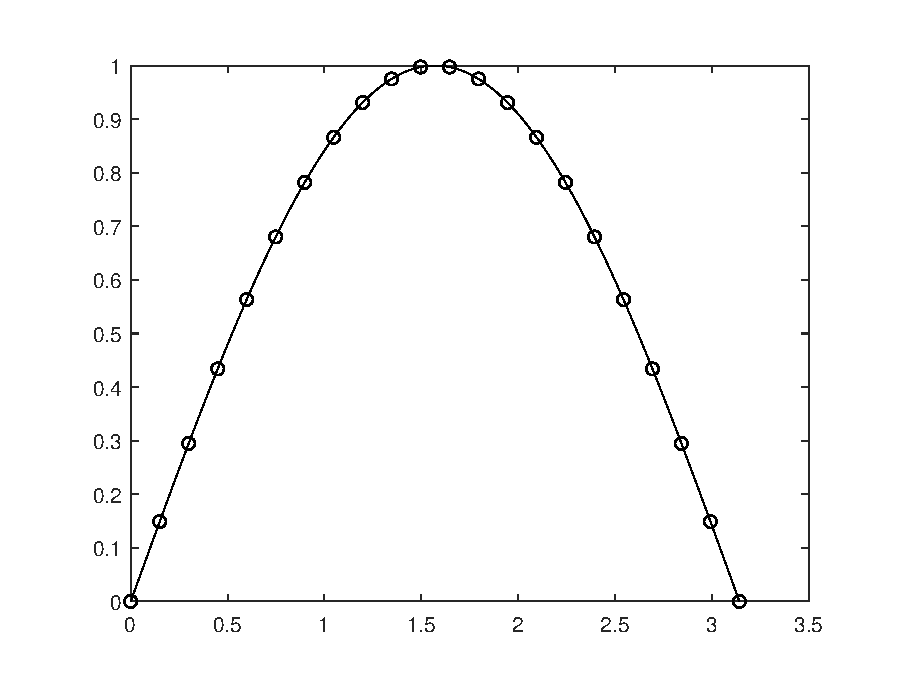
\includegraphics[scale=0.59]{e3_2_421.eps}
		}
		\caption{第3章 第2题 非扭结边界条件}
	\end{figure}

	\begin{figure}[htbp]
		\centering
		\subfigure[11个数据点及原曲线对比]{
			\includegraphics[scale=0.59]{e3_2_412.eps}
		} \quad
		\subfigure[21个数据点及原曲线对比]{
			\includegraphics[scale=0.59]{e3_2_422.eps}
		}
		\caption{第3章 第2题 非扭结边界条件及原曲线对比}
	\end{figure}
	
	由实验结果可以看到,在一般情况下,固定边界条件导致精度更高的近似,因为它包含关于函数的更多信息,但是为使这种边界条件成立,必须知道端点的导数值或对这些值的准确近似值。自然边界,非扭结边界的情况下拟合效果都比较好。效果最差的边界条件为周期边界,原因是周期边界的条件违背了原函数在两边端点处的导数性质。
	
	从11个数据点到21个数据点的结果对比来看,结果中函数并没有出现明显的震荡现象,这是因为使用了分片的思想,采用分段多项式插值。分段插值法通常有较好的收敛性和稳定性,且算法简单,但可能没有整体插值光滑,通过增加一些边界条件保证了区间端点的光滑性。
	
	不同的边界条件应该配合函数自身的性质使用,否则可能会造成较差的效果。
	
	\textit{Algorithm:}
	
	不同边界条件的矩阵已经从上一题中计算出,使用第6章中的方法求解线性方程组即可。
	
	\textit{Code:}
	
% -------------------------------代码----------------------------- %
\begin{lstlisting}[language = MATLAB]
function [a,b,c,d] = CubicSpline(n,x,a,fpo,fpv,mode)
% 样条插值
% mode:
% Nature 基于自然边界的样条函数
% Clamped 基于固定边界的样条函数
% Cycle 基于周期边界的样条函数
% Undistorted 基于非扭曲边界的样条函数
	h = zeros(n, 1);
	for i = 1:n
		h(i) = x(i+1) - x(i);
	end
	alpha = zeros(n+1, 1);
	for i = 2:n
		alpha(i) = 3 / h(i) * (a(i+1) - a(i)) - 3 / h(i-1) * (a(i) - a(i-1));
	end
	if mode == "Cycle"
		alpha(1) = (a(2) - a(1)) / h(1) - (a(n+1) - a(n)) / h(n);
	elseif mode == "Clamped"
		alpha(1) = 3 / h(1) * (a(2) - a(1)) - 3 * fpo;
		alpha(n+1) = 3 * fpv - 3 / h(n) * (a(n+1) - a(n));
	end
	A = zeros(n+1, n+1);
	for i = 2:n
		A(i, i-1) = h(i-1); A(i, i) = 2 * (h(i-1) + h(i)); A(i, i+1) = h(i);
	end
	if mode == "Nature"
		A(1, 1) = 1; A(n+1, n+1) = 1;
	elseif mode == "Cycle"
		A(1, 1) = 2 * h(1) / 3; A(1, 2) = h(1) / 3; A(1, n) = h(n) / 3; A(1, n+1) = 2 * h(n) / 3;
		A(n+1, 1) = 1; A(n+1, n+1) = -1;
	elseif mode == "Clamped"
		A(1, 1) = 2 * h(1); A(1, 2) = h(1);
		A(n+1, n) = h(n); A(n+1, n+1) = 2 * h(n);
	elseif mode == "Undistorted"
		A(1, 1) = h(2); A(1, 2) = -(h(1) + h(2)); A(1, 3) = h(1);
		A(n+1, n-1) = h(n); A(n+1, n) = -(h(n-1) + h(n)); A(n+1, n+1) = h(n-1);
	end
	[l, u, c] = LUDecomposition(n+1, A, alpha);
	b = zeros(n, 1); d = zeros(n, 1);
	for j = n:-1:1
		b(j) = (a(j+1) - a(j)) / h(j) - h(j) / 3 * (2 * c(j) + c(j+1));
		d(j) = (c(j+1) - c(j)) / (3 * h(j));
	end
	a = a(1:n)'; c = c(1:n);
end
\end{lstlisting}

调用该函数,根据不同的边界条件画图。

\begin{lstlisting}[language = MATLAB]
% 第3章 第2题
y = @(x)(sin(x));
N = 21; n = 20; x = 0 : pi/N : pi;
f = @(x, x0, a, b, c, d)(a + b * (x - x0) + c * (x - x0) .^ 2 + d * (x - x0) .^ 3);
mode = ["Nature", "Clamped", "Cycle", "Undistorted"];
color = ['g', 'r', 'b', 'k'];
for i = 2 : 2
	[a, b, c, d] = CubicSpline(N, x, y(x), cos(0), cos(pi), mode(i));
	for j = 1 : N
		x1 = x(j) : (x(j+1)-x(j))/n : x(j+1);
		plot(x1, f(x1, x(j), a(j), b(j), c(j), d(j)), color(i));
		hold on;
		scatter(x, y(x), color(i));
	end
end
hold on;
plot(0:pi / 1000:pi, y(0:pi / 1000:pi), 'c');
\end{lstlisting}
\newpage
	
\newpage
% --------------------------------第4章------------------------------- %
	\section{Chapter 4\quad 数值微分与数值积分}
	\label{sec:4}	
	
% ---------------------------实验题目 1.------------------------------- %
	\subsection{实验题目 1}
	\textit{Topic description:}
	
	推导复合(Composite)梯形公式及其误差估计;推导基于误差控制的逐次半积分梯形公式及其误差估计。
	
	\textit{Answer:}
	
	(1)\textbf{推导复合(Composite)梯形公式及其误差估计}:
	
	设$f\in C^2[a,b]$,将区间$[a,b]n$等分,步长$h=(b-a)/n$,$x_j=a+jh\quad(j=0,1,\dots,n)$,则
	\begin{equation*}
	\begin{split}
	\int_a^bf(x)dx&=\sum_{j=0}^{n-1}\int_{x_j}^{x_{j+1}}f(x)dx \\
	&=\sum_{j=0}^{n-1}\{\frac{h}{2}[f(x_j)+f(x_{j+1})]-\frac{h^3}{12}f^{''}(\xi_j)\} \\
	&=\frac{h}{2}\sum_{j=0}^{n-1}[f(x_j)+f(x_{j+1})]-\frac{h^3}{12}\sum_{j=0}^{n-1}f^{''}(\xi_j),\xi_j\in (x_j,x_{j+1})
	\end{split}
	\end{equation*}
	
	因此梯形公式为
	\begin{equation*}
	T_n=\frac{h}{2}[f(a)+2\sum_{j=1}^{n-1}+f(b)]
	\end{equation*}
	
	误差估计为
	\begin{equation*}
	E(f)=-\frac{h^3}{12}\sum_{j=0}^{n-1}f^{''}(\xi_j)
	\end{equation*}
	
	因为$f\in C^2[a,b]$,由闭区间上连续函数的介值定理知,存在$\mu\in(a,b)$使得$f^{''}(\mu)=\frac{1}{n}\sum_{j=0}^{n-1}f^{''}(\xi_j)$,因此
	\begin{equation*}
	E(f)=-\frac{h^3}{12}nf^{''}(\mu)=-\frac{b-a}{12}h^2f^{''}(\mu),\mu\in(a,b)
	\end{equation*}
	
	(2)\textbf{推导基于误差控制的逐次半积分梯形公式及其误差估计}:
	
	令$h_n=\frac{b-a}{n}$,则根据复合梯形公式
	\begin{equation*}
	\begin{split}
	\int_a^bf(x)dx&=\frac{h_n}{2}[f(a)+2\sum_{j=1}^{n-1}f(x_j)+f(b)]-\frac{b-a}{12}h_n^2f^{''}(\mu) \\
	&=S_n-\frac{b-a}{12}h_n^2f^{''}(\mu)
	\end{split}
	\end{equation*}
	其中$S_n=\frac{h_n}{2}[f(a)+2\sum\limits_{j=1}^{n-1}f(x_j)+f(b)]$。
	
	令$h_{2n}=\frac{b-a}{2n}=\frac{h_n}{2}$,同样地
	\begin{equation*}
	\begin{split}
	\int_a^bf(x)dx&=\frac{h_{2n}}{2}[f(a)+2\sum_{j=1}^{2n-1}f(x_j)+f(b)]-\frac{b-a}{12}h_{2n}^2f^{''}(\widetilde\mu) \\
	&=S_{2n}-\frac{b-a}{12}h_{2n}^2f^{''}(\widetilde\mu)
	\end{split}
	\end{equation*}
	其中$S_{2n}=\frac{h_{2n}}{2}[f(a)+2\sum\limits_{j=1}^{2n-1}f(x_j)+f(b)]$。
	\begin{equation*}
	\int_a^bf(x)dx=S_n-\frac{b-a}{12}h_n^2f^{''}(\mu)=S_{2n}-\frac{b-a}{12}h_{2n}^2f^{''}(\widetilde\mu)
	\end{equation*}
	
	假设$\mu\approx\widetilde\mu$,即$f^{''}(\mu)\approx f^{''}(\widetilde\mu)$,可得
	\begin{equation*}
	S_n-\frac{b-a}{12}h_n^2f^{''}(\mu)\approx S_{2n}-\frac{1}{4}\cdot\frac{b-a}{12}h_{n}^2f^{''}(\mu)
	\end{equation*}
	即
	\begin{equation*}
	\frac{b-a}{12}h_n^2f^{''}(\mu)=\frac{4}{3}[S_n-S_{2n}]
	\end{equation*}
	我们得到
	\begin{equation*}
	\int_a^bf(x)dx-S_{2n}\approx\frac{1}{3}[S_n-S_{2n}]
	\end{equation*}
	给定误差$\varepsilon$,如果$|S_n-S_{2n}|<3\varepsilon$,则$|\int_a^bf(x)dx-S_{2n}|<\varepsilon$
	
% ----------------------------实验题目 2.------------------------------ %
	\subsection{实验题目 2}
	\textit{Topic description:}
	
	let $h=(b-a)/3,x_0=a,x_1=a+h,x_2=b$.Find the degree of precision of the quadrature formula
	\begin{equation*}
	\int_{a}^{b}f(x)dx=\frac{9}{4}hf(x_1)+\frac{3}{4}hf(x_2).
	\end{equation*}
	
	\textit{Answer:}
	
	分别将$f(x)=1,x,x^2,x^3$带入求积公式,可以令$a=0,b=3$,则$h=1,x_0=0,x_1=1,x_2=3$
	
	当$f(x)=1$时
	
	$\int_{a}^{b}f(x)dx=\int_{0}^{3}1dx=3$,而$\frac{9}{4}hf(x_1)+\frac{3}{4}hf(x_2)=\frac{9}{4}+\frac{3}{4}=3$,二者相等。
	
	当$f(x)=x$时
	
	$\int_{a}^{b}f(x)dx=\int_{0}^{3}xdx=\frac{9}{2}$,而$\frac{9}{4}hf(x_1)+\frac{3}{4}hf(x_2)=\frac{9}{4}+\frac{9}{4}=\frac{9}{2}$,二者相等。
	
	当$f(x)=x^2$时
	
	$\int_{a}^{b}f(x)dx=\int_{0}^{3}x^2dx=9$,而$\frac{9}{4}hf(x_1)+\frac{3}{4}hf(x_2)=\frac{9}{4}+\frac{27}{4}=9$,二者相等。
	
	当$f(x)=x^3$时
	
	$\int_{a}^{b}f(x)dx=\int_{0}^{3}x^3dx=\frac{81}{4}$,而$\frac{9}{4}hf(x_1)+\frac{3}{4}hf(x_2)=\frac{9}{4}+\frac{81}{4}=\frac{90}{4}$,二者不相等。
	
	在$f(x)=1,x,x^2$时二者相等,$f(x)=x^3$时不相等,因此精度为2。
	
% ----------------------------实验题目 3.------------------------------ %
	\subsection{实验题目 3}
	\textit{Topic description:}
	
	自行编制复合梯形公式、Simpson公式的计算程序;
	
	取$h=0.01$,分别利用复合梯形、Simpson公式计算定积分
	\begin{equation*}
	I(f)=\frac{1}{\sqrt{2\pi}}\int_0^1exp^{-\frac{x^2}{2}}dx
	\end{equation*}
	
	试与精确解比较,说明两种格式的优劣
	
	若取计算精度为$10^{-4}$,则$h=?,n=?$
	
	\textit{Answer:}
	
	精确解为0.341344746068543
	\begin{table}[htbp]
		\centering
		\caption{第4章 第3题 近似解}\label{e4_3_1}
		\begin{tabular}
			{c|c|c}
			\hline
			&近似解&误差 \\
			\hline
			复合梯形公式&0.341342729639117&2.0164e-06 \\
			\hline
			复合Simpson公式&0.341344746095430&2.6887e-11 \\
			\hline
		\end{tabular}
	\end{table}
	
	\begin{table}[htbp]
		\centering
		\caption{第4章 第3题 h与n的取值}\label{e4_3_2}
		\begin{tabular}
			{c|c|c}
			\hline
			&h&n \\
			\hline
			复合梯形公式&0.0667&15 \\
			\hline
			复合Simpson公式&0.25&4 \\
			\hline
		\end{tabular}
	\end{table}
	
	由表(\ref{e4_3_1})可知,复合Simpson公式的误差比复合梯形公式要小得多,两者相差多个数量级。在理论上复合梯形公式的精度为1次,Simpson公式的精度为3次,且两种算法的计算量大致相同。在实际计算结果中Simpson公式也取得了更高的精度。
	
	由表(\ref{e4_3_2})可知,在计算精度为$10^{-4}$的情况下,复合Simpson公式的n比复合梯形公式要少,复合Simpson公式的h仅在复合梯形公式的h近4倍的情况下达到了相同的精度。
	
	\textit{algorithm:}
	
	\begin{algorithm}
		\caption{Composite Trapezoidal's Rule}
		\KwIn{endpoints $a,b$; even positive integer $n$}
		\KwOut{approximation $XI$ to $I$}
		Set $h=(b-a)/n;$
		
		Set $XI0=f(a)+f(b); XI1=0;$
		
		\For{$i=1,2,\dots,n-1$}
		{
			Set $X=a+ih;$
			
			Set $XI1=XI1+f(X);$
		}
		
		Set $XI=h(XI0+2XI1)/2;$
		
		OUTPUT($XI$);(Procedure completed successfully)
		
		STOP;
	\end{algorithm}
	
	\begin{algorithm}
		\caption{Composite Simpson's Rule}
		\KwIn{endpoints $a,b$; even positive integer $n$}
		\KwOut{approximation $XI$ to $I$}
		Set $h=(b-a)/n;$
		
		Set $XI0=f(a)+f(b); XI1=0; XI2=0;$
		
		\For{$i=1,2,\dots,n-1$}
		{
			Set $X=a+ih;$
			
			\If{$i$ is even}{
				Set $XI2=XI2+f(X);$
			}
			\Else
			{
				Set $XI1=XI1+f(X);$
			}
		}
	
		Set $XI=h(XI0+2XI2+4XI1)/3;$
		
		OUTPUT($XI$);(Procedure completed successfully)
		
		STOP;
	\end{algorithm}
	
	\textit{Code:}
	
% ----------------------------------代码-------------------------------- %
\begin{lstlisting}[language = MATLAB]
function [XI] = CompositeTrapezoidal(a,b,n,f)
% 复合梯形
	h = (b - a) / n;
	XI0 = f(a) + f(b); XI1 = 0;
	for i = 1:n-1
		X = a + i * h;
		XI1 = XI1 + f(X);
	end
	XI = h * (XI0 + 2 * XI1) / 2;
end
\end{lstlisting}

\begin{lstlisting}[language = MATLAB]
function [XI] = CompositeSimpson(a,b,n,f)
% 复合Simpson
	h = (b - a) / n; XI0 = f(a) + f(b);
	XI1 = 0;  %odd
	XI2 = 0;  %even
	for i = 1:n-1
		X = a + i * h;
		if mod(i, 2) == 1
			XI1 = XI1 + f(X);
		else
			XI2 = XI2 + f(X);
		end
	end
	XI = h * (XI0 + 2 * XI2 + 4 * XI1) / 3;
end
\end{lstlisting}

\begin{lstlisting}[language = MATLAB]
function [h,n] = ComputeH(tol,method,a,b,f,I)
% 给定计算精度,计算h与n
	maxH = 200;
	for n = 1 : maxH
		h = (b - a) / n;
		if method == "CompositeTrapezoidal"
			I1 = CompositeTrapezoidal(a, b, n, f) / sqrt(2 * pi);
		elseif method == "CompositeSimpson"
			I1 = CompositeSimpson(a, b, n, f) / sqrt(2 * pi);
		end
		if abs(I1 - I) <= tol
			break;
		end
	end
end
\end{lstlisting}

\begin{lstlisting}[language = MATLAB]
% 第4章 第3题
f = @(x)(exp(-x^2 / 2));
a = 0; b = 1; h = 0.01; n = (b - a) / h;
I1 = CompositeTrapezoidal(a, b, n, f) / sqrt(2 * pi);  % 复合梯形
I2 = CompositeSimpson(a, b, n, f) / sqrt(2 * pi);  % 复合simpson
s = @(x)((2^(1/2)*pi^(1/2)*erf((2^(1/2)*x)/2))/2);  % 积分后的原函数
I = (s(b) - s(a)) / sqrt(2 * pi);  % 精确解
[h1, n1] = ComputeH(1e-4, "CompositeTrapezoidal", a, b, f, I);
[h2, n2] = ComputeH(1e-4, "CompositeSimpson", a, b, f, I);
\end{lstlisting}

% ----------------------------实验题目 4.-------------------------------- %
	\subsection{实验题目 4}
	\textit{Topic description:}
	
	分别利用复合梯形、Simpson公式计算定积分
	\begin{equation*}
	I(f)=\int_1^6(2+\sin(2\sqrt{x}))dx
	\end{equation*}
	
	取$h=0.5,0.25,0.125$,列表给出两种格式的近似计算结果。
	
	\textit{Answer:}
	
	精确解为8.1835
	
	\begin{table}[htbp]
		\centering
		\caption{第4章 第4题 近似计算结果}\label{e4_4}
		\begin{tabular}
			{c|c|c|c|c}
			\hline
			h&复合梯形公式近似解&复合梯形公式误差&复合Simpson公式近似解&复合Simpson公式误差 \\
			\hline
			0.5&8.1939&0.0104&8.1830&4.6371e-04 \\
			\hline
			0.25&8.1860&0.0026&8.1834&3.1711e-05 \\
			\hline
			0.125&8.1841&6.4098e-04&8.1835&2.0399e-06 \\
			\hline
		\end{tabular}
	\end{table}

	从表(\ref{e4_4})种可以看出,随着h减小,近似解与精确解的误差不断减少,在相同 的h下,复合Simpson公式近似解要比复合梯形公式近似解的误差更小。

	\textit{Code:}
	
% ----------------------------------代码-------------------------------- %
\begin{lstlisting}[language = MATLAB]
% 第4章 第4题
a = 1; b = 6; hs = [0.5, 0.25, 0.125];
f = @(x)(2 + sin(2 * sqrt(x)));
I1 = zeros(3, 1); I2 = zeros(3, 1);
s = @(x)(2*x + sin(2*x^(1/2))/2 + x^(1/2)*(2*sin(x^(1/2))^2 - 1));
I = s(b) - s(a);
for i = 1:3
	h = hs(i);
	n = (b - a) / h;
	I1(i) = CompositeTrapezoidal(a, b, n, f);
	I2(i) = CompositeSimpson(a, b, n, f);
end
\end{lstlisting}

\newpage
	
	
\newpage
% --------------------------------第5章------------------------------- %
	\section{Chapter 5\quad 常微分方程数值解}
	\label{sec:5}	
	
% ----------------------------实验题目 1.------------------------------ %
	\subsection{实验题目 1}
	\textit{Topic description:}
	
	求$y^{'}=1+y²,y(0)=0$的数值解(分别用欧拉显格式、梯形预估修正格式、4阶龙格库塔格式,并与解析解比较这三种格式的收敛性)。
	
	\textit{Answer:}
	
	\textbf{欧拉显格式}:
	
	Euler法的目的是获得适定的初值问题$$\frac{dy}{dt}=f(t,y),\quad a\leq t\leq b,\quad y(a)=\alpha$$的近似解。
	
	规定网格点在区间$[a,b]$是均等分布的。为保证此条件,选择一个正整数$N$,并选取网格点$$t_i=a+ih,\quad i=0,1,2,\dots,N$$网格点之间的普通距离$h=(b-a)/N$称为步长。
	
	使用Taylor定理推导Euler法。假设唯一解$y(t)$在$[a,b]$上具有二阶连续导数,对$i=0,1,2,\dots,N-1$,有$$y(t_{i+1})=y(t_i)+(t_{i+1}-t_i)y^{'}(t_i)+\frac{(t_{i+1}-t_i)^2}{2}y^{''}(\xi_i)$$对$(t_i,t_{i+1})$内的某点$\xi_i$成立。因为$h=t_{i+1}-t_i$,所以有
	\begin{equation*}
	\begin{aligned}
	y(t_{i+1})&=y(t_i)+hy^{'}(t_i)+\frac{h^2}{2}y^{''}(\xi_i) \\
	&=y(t_i)+hf(t_i,y(t_i))+\frac{h^2}{2}y^{''}(\xi_i)
	\end{aligned}
	\end{equation*}
	
	Euler法通过消去余项构造$w_i\approx y(t_i)(i=1,2,\dots,N)$。因而Euler法为
	\begin{equation*}
	\begin{aligned}
	w_0&=\alpha \\
	w_{i+1}&=w_i+hf(t_i,w_i),\quad i=0,1,\dots,N-1
	\end{aligned}
	\end{equation*}
	
	\textbf{梯形预估修正格式}:
	
	使用Euler显格式
	\begin{equation*}
	\begin{aligned}
	y_0&=\alpha \\
	y_{i+1}&=y_i+hf(t_i,y_i),\quad i=0,1,\dots,N-1
	\end{aligned}
	\end{equation*}
	
	做预估,梯形公式$$y_{i+1}=y_i+\frac{h}{2}[f(t_i,y_i)+f(t_{i+1},y_{i+1})]$$做修正,计算公式为
	
	\begin{equation*}
	\begin{aligned}
	y_0&=\alpha \\
	y_{i+1}=y_i+\frac{h}{2}[f(t_i,y_i)+f(t_{i+1},y_i+hf(t_i,y_i))],\quad i=0,1,\dots,N-1
	\end{aligned}
	\end{equation*}
	
	\textbf{4阶龙格库塔格式}:
	
	4阶Runge-Kutta方法:
	\begin{equation*}
	\begin{aligned}
	w_0&=\alpha \\
	k_1&=hf(t_i,w_i) \\
	k_2&=hf(t_i+\frac{h}{2},w_i+\frac{1}{2}k_1) \\
	k_3&=hf(t_i+\frac{h}{2},w_i+\frac{1}{2}k_2) \\
	k_4&=hf(t_{i+1},w_i+k_3) \\
	w_{i+1}&=w_i+\frac{1}{6}(k_1+2k_2+2k_3+k_4)
	\end{aligned}
	\end{equation*}
	
	对每一个$i=0,1,\dots,N-1$成立。这个方法具有局部截断误差$O(h^4)$,只要解$y(t)$具有5阶连续导数。
	
	\begin{figure}[htbp]
		\centering
		\subfigure[欧拉显格式]{
			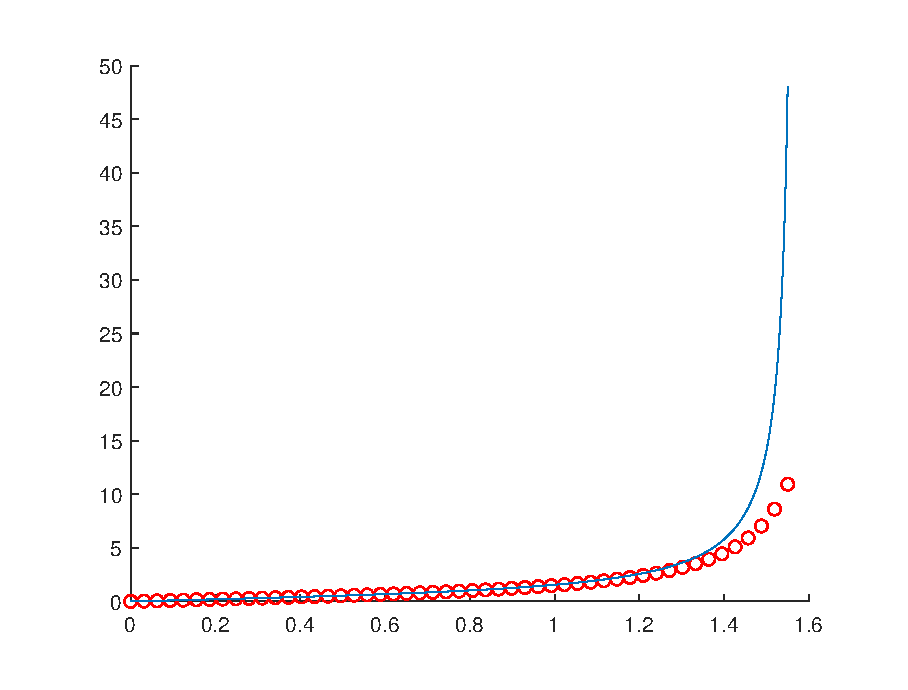
\includegraphics[scale=0.6]{e5_1_x1.eps}
		} \quad
		\subfigure[梯形预估修正格式]{
			\includegraphics[scale=0.6]{e5_1_x2.eps}
		} \quad
		\subfigure[4阶龙格库塔格式]{
			\includegraphics[scale=0.6]{e5_1_x3.eps}
		}\caption{第5章 第1题 $y^{'}=1+y²,y(0)=0$不同方法数值解}
	\end{figure}
	
	\begin{figure}[htbp]
		\centering
		\includegraphics[scale=0.8]{e5_1_x.eps}
		\caption{第5章 第1题 $y^{'}=1+y²,y(0)=0$三种方法对比}\label{e5_1}
	\end{figure}
	
	通过图(\ref{e5_1})与解析解(曲线)对比可以看出三种格式的收敛性对比为:欧拉显格式$<$梯形预估修正格式$<$4阶龙格库塔格式。
	
	\textit{algorithm:}
	
	\begin{algorithm}
		\caption{Euler' Method}
		\KwIn{endpoints $a,b$; integer $N$; initial condition $\alpha$;}
		\KwOut{approximation $w$ to $y$ at $N+1$ points of $t$}
		Set $h=(b-a)/N; t=a; w=\alpha;$
		
		OUTPUT($t,w$);
		
		\For{$i=1,2,\dots,N$}
		{
			Set $w=w+hf(t,w); t=a+ih;$
			
			OUTPUT($t,w$);
		}
		
		STOP;
	\end{algorithm}

	\begin{algorithm}
		\caption{Runge-Kutta(Order Four)}
		\KwIn{endpoints $a,b$; integer $N$; initial condition $\alpha$;}
		\KwOut{approximation $w$ to $y$ at $N+1$ points of $t$}
		Set $h=(b-a)/N; t=a; w=\alpha;$
		
		OUTPUT($t,w$);
		
		\For{$i=1,2,\dots,N$}
		{
			Set $K_1=hf(t,w),K_2=hf(t+\frac{h}{2},w+\frac{1}{2}K_1),K_3=hf(t+\frac{h}{2},w+\frac{1}{2}K_2),K_4=hf(t+h,w+K_3);$
			
			Set $w=w+\frac{1}{6}(K_1+2K_2+2K_3+K_4); t=a+ih;$
			
			OUTPUT($t,w$);
		}
		
		STOP;
	\end{algorithm}
	
	\textit{Code:}
	
% ----------------------------------代码-------------------------------- %
\begin{lstlisting}[language = MATLAB]
function [t,w] = EulerMethod(a,b,N,alpha,f)
% 欧拉显格式
	h = (b - a) / N;
	t = zeros(N+1, 1);
	w = zeros(N+1, 1);
	t(1) = a; w(1) = alpha;
	for iter = 1:N
		w(iter+1) = w(iter) + h * f(t(iter), w(iter));
		t(iter+1) = a + iter * h;
	end
end
\end{lstlisting}

\begin{lstlisting}[language = MATLAB]
function [t,w] = TrapezoidalPredictorCorrector(a,b,N,alpha,f)
% 梯形预估修正格式
	h = (b - a) / N;
	t = zeros(N+1, 1);
	w = zeros(N+1, 1);
	t(1) = a; w(1) = alpha;
	for iter = 1:N
		t(iter+1) = a + iter * h;
		w(iter+1) = w(iter) + h/2*(f(t(iter),w(iter))+f(t(iter+1),w(iter)+h*f(t(iter),w(iter))));
	end
end
\end{lstlisting}

\begin{lstlisting}[language = MATLAB]
function [t,w] = RungeKuttaOrder4(a,b,N,alpha,f)
% 4阶龙格库塔方法
	h = (b - a) / N;
	t = zeros(N+1, 1);
	w = zeros(N+1, 1);
	t(1) = a; w(1) = alpha;
	for iter = 1:N
		K1 = h * f(t(iter), w(iter));
		K2 = h * f(t(iter) + h/2, w(iter) + K1/2);
		K3 = h * f(t(iter) + h/2, w(iter) + K2/2);
		K4 = h * f(t(iter) + h, w(iter) + K3);
		w(iter+1) = w(iter) + (K1 + 2*K2 + 2*K3 + K4) / 6;
		t(iter+1) = a + iter * h;
	end
end
\end{lstlisting}

\begin{lstlisting}[language = MATLAB]
% 第5章 第1题
f = @(t,y)(1 + y ^ 2);
a = 0; b = 1.55; N = 50; alpha = 0;
[t,w] = EulerMethod(a,b,N,alpha,f);
scatter(t, w, 'r');
hold on;
[t,w] = TrapezoidalPredictorCorrector(a,b,N,alpha,f);
scatter(t, w, 'b');
hold on;
[t,w] = RungeKuttaOrder4(a,b,N,alpha,f);
scatter(t, w, 'g');
hold on;
s = @(t)(tan(t));
t = a:(b-a)/(N*100):b;
w = s(t);
plot(t, w);
legend('Euler Method', 'Trapezoidal Predictor-Corrector', 'Runge-Kutta Order 4', 'y(x)', 'Location', 'northwest');
\end{lstlisting}
	
% ----------------------------实验题目 2.-------------------------------- %
	\subsection{实验题目 2}
	\textit{Topic description:}
	
	用龙格库塔4阶方法求解描述振荡器的经典的Van der Pol微分方程
	\begin{equation*}
	\left\{
	\begin{aligned}
	&\frac{d^2 y}{dt^2}-\mu(1-y^2)\frac{dy}{dt}+y=0, \\
	&y(0)=1,y^{'}(0)=0.
	\end{aligned}
	\right.
	\end{equation*}
	
	分别取$\mu=0.01,0.1,1$,作图比较计算结果。
	
	\textit{Answer:}
	
	\begin{figure}[htbp]
		\centering
		\subfigure[$\mu=0.01\quad b=10$]{
			\includegraphics[scale=0.28]{e5_2_x10.jpg}
		} \quad
		\subfigure[$\mu=0.1\quad b=10$]{
			\includegraphics[scale=0.28]{e5_2_x20.jpg}
		} \quad
		\subfigure[$\mu=1\quad b=10$]{
			\includegraphics[scale=0.28]{e5_2_x30.jpg}
		}
		\subfigure[$\mu=0.01\quad b=100$]{
			\includegraphics[scale=0.28]{e5_2_x11.jpg}
		} \quad
		\subfigure[$\mu=0.1\quad b=100$]{
			\includegraphics[scale=0.28]{e5_2_x21.jpg}
		} \quad
		\subfigure[$\mu=1\quad b=100$]{
			\includegraphics[scale=0.28]{e5_2_x31.jpg}
		}
		\subfigure[$\mu=0.01\quad b=300$]{
			\includegraphics[scale=0.28]{e5_2_x12.jpg}
		} \quad
		\subfigure[$\mu=0.1\quad b=300$]{
			\includegraphics[scale=0.28]{e5_2_x22.jpg}
		} \quad
		\subfigure[$\mu=1\quad b=300$]{
			\includegraphics[scale=0.28]{e5_2_x32.jpg}
		}
		\caption{第5章 第2题 Van der Pol微分方程}\label{e5_2}
	\end{figure}
	
	如图(\ref{e5_2})所示,在尺度很小的情况下观察时,随着$\mu$变大,感觉曲线变形得越厉害。尺度放大一些,发现$\mu$取这3个值时,曲线都在变形,不过$\mu$越大,变形得越快,相应的也很快达到了一种平衡。
	
	\textit{Code:}

% --------------------------------代码----------------------------------- %
\begin{lstlisting}[language = MATLAB]
function [w] = RungeKutta2(a,b,m,N,alpha,f)
% 微分方程组的Runge_Kutta方法
	h = (b - a) / N;
	t = a;
	w = zeros(N+1, m);
	for i = 1:m
		w(1, i) = alpha(i);  % 初值条件
	end
	for i = 1:N-1
		k1 = zeros(m, 1); k2 = zeros(m, 1); k3 = zeros(m, 1); k4 = zeros(m, 1);
		for j = 1:m
			k1(j) = h * f{j}(t, w(i, :)');
		end
		for j = 1:m
			k2(j) = h * f{j}(t+h/2, w(i, :)'+k1/2);
		end
		for j = 1:m
			k3(j) = h * f{j}(t+h/2, w(i, :)'+k2/2);
		end
		for j = 1:m
			k4(j) = h * f{j}(t+h, w(i, :)'+k3);
		end
		for j = 1:m
			w(i+1, j) = w(i, j) + (k1(j)+2*k2(j)+2*k3(j)+k4(j)) / 6;
		end
		t = t + h;
	end
end
\end{lstlisting}

\begin{lstlisting}[language = MATLAB]
% 第5章 第2题
mu = 0.01;  % [0.01, 0.1, 1]
f = {@(t, w)(w(2)), @(t, w)(mu*(1-w(1)*w(1))*w(2)-w(1))};
a = 0; b = 300; m = 2; N = 10000; alpha = [1, 0];
w = RungeKutta2(a,b,m,N,alpha,f);
plot(a:(b-a)/N:b, w(:, 1)');
\end{lstlisting}

% ----------------------------实验题目 3.-------------------------------- %
	\subsection{实验题目 3}
	\textit{Topic description:}
	
	试用Adams Fourth-Order Predictor-Corrector格式(原书P311)求解如下常微分方程初值问题
	\begin{equation*}
	\left\{
	\begin{aligned}
	&\frac{dy}{dt}=\frac{t-y}{2},0\leq x\leq 3; \\
	&y(0)=1.
	\end{aligned}
	\right.
	\end{equation*}
	
	的数值解(分别取h=1,0.5,0.25,0.125)
	
	\textit{Answer:}
	
	显式和隐式方法的组合称作预测校正法。显式方法预测逼近值,隐式方法校正此预测。
	
	\textbf{Adams4阶预测修正法}第一步是对于4步显式Adams-Bashforth方法计算初始值$w_0,w_1,w_2$和$w_3$。为此,使用4阶单步法,即4阶Runge-Kutta方法。下一步是计算$y(t_4)$的近似值$w_4^{(0)}$,使用显式Adams-Bashforth 方法作为预测值:$$w_4^{(0)}=w_3+\frac{h}{24}[55f(t_3,w_3)-59f(t2,w2)+37f(t_1,w_1)-9f(t_0,w_0)]$$此近似值可以通过将$w_4^{(0)}$插入到三步隐式Adams-Moulton方法的右端且使用该方法作为一个校正来改进。由此得到$$w_4^{(1)}=w_3+\frac{h}{24}[9f(t_4,w_4^{(0)})+19f(t_3,w_3)-5f(t_2,w_2)+f(t_1,w_1)]$$在这个过程中所需的唯一新函数求值是校正方程中的$f(t_4,w_4^{(0)})$;所有其他的$f$值已经对于以前的近似值计算出来。
	
	值$w_4^{(1)}$用作$y(t_4)$的近似值,重复使用Adams-Bashforth方法作为预测值和Adams-Moulton方法作为校正的技术以求出$y(t_5)$的最初和最终近似值$w_5^{(0)}$和$w_5^{(1)}$,等等。
	
	\begin{figure}[htbp]
		\centering
		\subfigure[$h=1$]{
			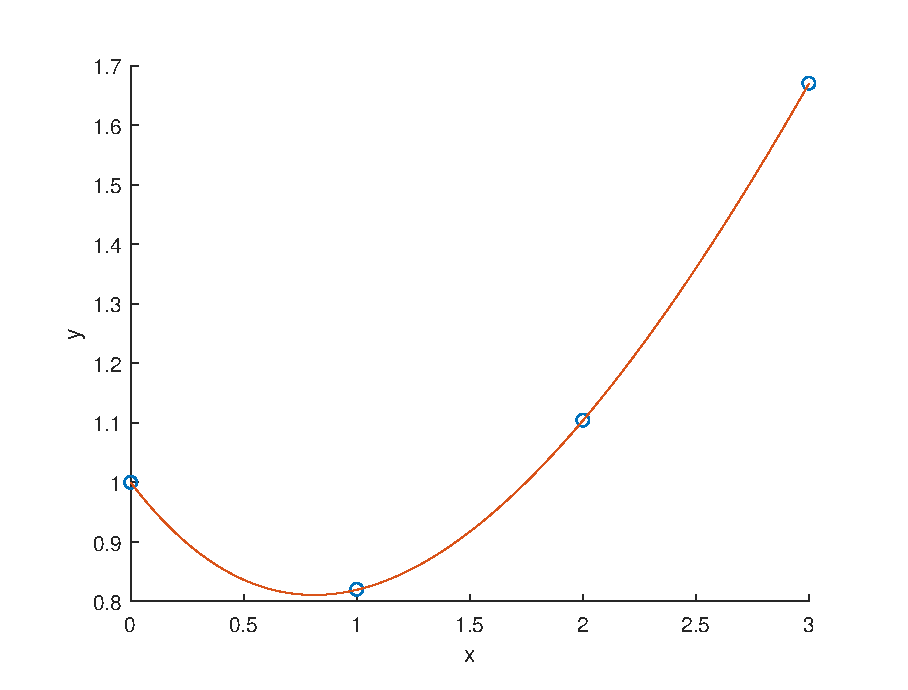
\includegraphics[scale=0.59]{e5_3_x1.eps}
		} \quad
		\subfigure[$h=0.5$]{
			\includegraphics[scale=0.59]{e5_3_x2.eps}
		} \quad
		\subfigure[$h=0.25$]{
			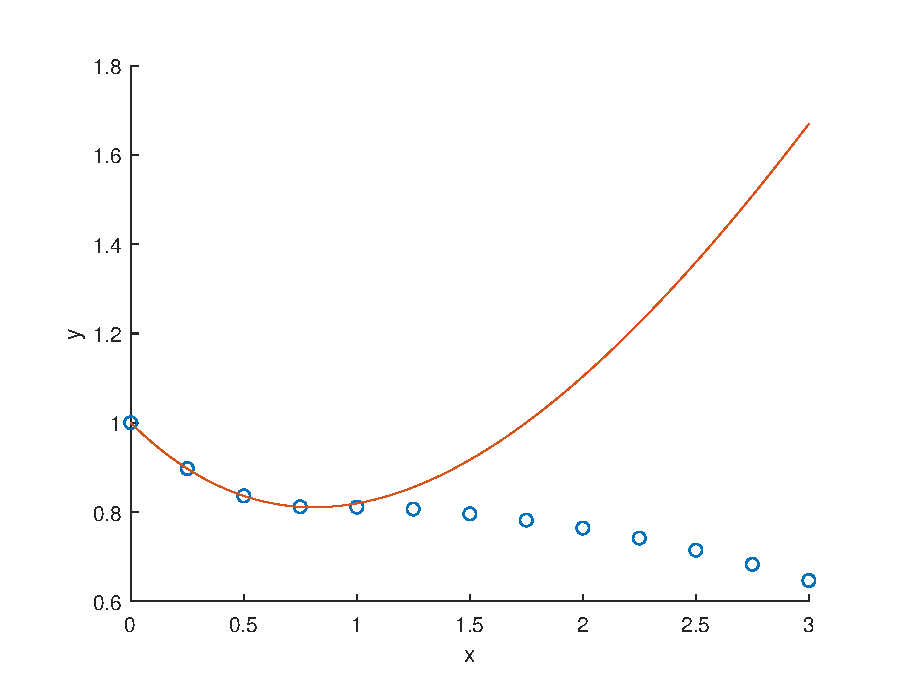
\includegraphics[scale=0.59]{e5_3_x3.eps}
		} \quad
		\subfigure[$h=0.125$]{
			\includegraphics[scale=0.59]{e5_3_x4.eps}
		} \quad
		\subfigure[$h=1,0.5,0.25,0.125$]{
			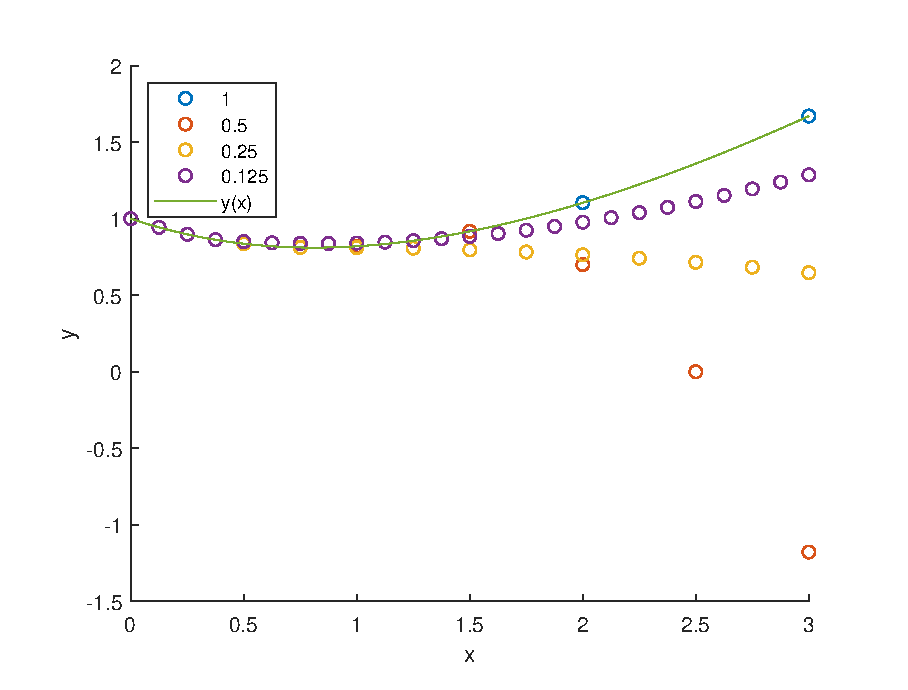
\includegraphics[scale=0.59]{e5_3_x.eps}
		}
		\caption{第5章 第3题 Adams Fourth-Order Predictor-Corrector近似解}\label{e5_3}
	\end{figure}
	
	由图(\ref{e5_3})可以发现:$h=1$时4个数值解都在解析解曲线上,拟合的很好,但继续观察发现,$h$取不同数值时前4个数据点都拟合的非常好,且落在解析解曲线上,随着$h$值不断减小,数值解的走势与数值不断与解析解靠拢,可以直观地想到:随着$h$越来越小,划分的区间数量$n$越来越多,拟合的也会越来越精确。
	
	\textit{Code:}
	
% --------------------------------代码----------------------------------- %
\begin{lstlisting}[language = MATLAB]
% 第5章 第3题
f = @(t, y)((t - y) / 2);
a = 0; b = 3; alpha = 1;
for h = [1, 0.5, 0.25, 0.125]
	[t, w] = AdamsFourthOrderPredictorCorrector(a, b, (b - a) / h, alpha, f);
	scatter(t, w);
	hold on;
end
s = @(t)(t + 3*exp(-t/2) - 2);
t = a:0.01:b;
w = s(t);
plot(t, w);
xlabel("x");
ylabel("y");
legend('1', '0.5', '0.25', '0.125', 'y(x)', 'Location', 'NorthWest');
\end{lstlisting}
	
\newpage

\newpage
% --------------------------------第6,7章-------------------------------- %
	\section{Chapter 6,7\quad 线性方程组求解}
	\label{sec:6}
	
% ----------------------------实验题目 1.-------------------------------- %
	\subsection{实验题目 1}
	\textit{Topic description:}
	
	求解线性方程组
	\begin{equation*}
	\left\{
	\begin{aligned}
	4x-y+z&=7 \\
	4x-8y+z&=-21 \\
	-2x+y+5z&=15
	\end{aligned}
	\right.
	\end{equation*}
	
	(1)试用LU分解求解此方程组
	
	(2)分别用Jacobi,Gauss-Seidel方法求解此方程组
	
	\textit{Answer:}
	
	(1)\textbf{LU分解}:设无行交换变换的高斯消去法可解一般线性方程组$Ax=b$,则矩阵$A$可分解为一个下三角矩阵和一个上三角矩阵的乘积:
	\begin{equation*}
	A=LU
	\end{equation*}
	
	其中$L$的对角线元素为1,$U$的对角线元素非零。此时$LUx=b$,令$y=Ux$,然后通过以下步骤求解$x$:
	
	a)使用前向替换法求解方程组$Ly=b$得到$y$
	
	b)使用回代法求解方程组$Ux=y$得到$x$
	
	(2)设有如下方程组:
	\begin{equation*}
	\left\{
	\begin{aligned}
	a_{11}x_1+a_{12}x_2+\dots+a_{1n}x_n&=b_1 \\
	a_{21}x_1+a_{22}x_2+\dots+a_{2n}x_n&=b_2 \\
	\vdots& \\
	a_{n1}x_1+a_{n2}x_2+\dots+a_{nn}x_n&=b_n
	\end{aligned}
	\right.
	\end{equation*}
	
	\textbf{Jacobi方法}:迭代方法将线性方程组$Ax=b$转换为具有$x=Tx+c$($T$为定常矩阵$c$为定常向量)形式的等价方程组,给定解$x$的初始近似值,然后产生收敛于$x$的向量序列$\{x^{(k)}\}_{k=0}^\infty$。
	
	Jacobi迭代法包含了从$Ax=b$中的第$i$个方程求解第$i$个分量$x_i$,得到(假设$a_{ii}\neq 0$)
	\begin{equation*}
	x_i=\sum_{j=1,j\neq i}^{n}(-\frac{a_{ij}x_j}{a_{ii}})+\frac{b_i}{a_{ii}},\quad i=1,2,\dots,n
	\end{equation*}
	
	以及当$k\geq 1$时,从分量$x^{(k-1)}$计算生成各个$x_i^{(k)}$
	\begin{equation*}
	x_i^{(k)}=\frac{\sum_{j=1,j\neq i}^{n}(-a_{ii}x_j^{(k-1)})+b_i}{a_{ii}},\quad i=1,2,\dots,n
	\end{equation*}
	
	\textbf{Gauss-Seidel方法}:对Jacobi迭代法的一种改进。$x^{(k-1)}$的分量可以用来计算$x_i^{(k)}$,因为对$i>1,x_1^{(k)},\dots,x_{i-1}^{(k)}$已经计算出来了,并且可能比$x_1^{(k-1)},\dots,x_{i-1}^{(k-1)}$更接近于实际解,显然使用那些新近计算出来的值来计算$x_i^{(k)}$更合理。
	\begin{equation*}
	x_i^{(k)}=\frac{-\sum\limits_{j=1}^{i-1}(a_{ij}x_j^{(k)})-\sum\limits_{j=i+1}^{n}(a_{ij}x_j^{(k-1)})+b_i}{a_{ii}},\quad i=1,2,\dots,n
	\end{equation*}
	
	LU分解得出的解为$x=2,y=4,z=3$
	
	\begin{table}[htbp]
		\centering
		\caption{求解线性方程组精度为1e-5时结果}\label{e6_1}
		\begin{tabular}
			{c|c|c}
			\hline
			&Jacobi&Gauss-Seidel \\
			\hline
			$x$&1.9995&1.9999 \\
			\hline
			$y$&3.9998&3.9999 \\
			\hline
			$z$&3.0002&3.0000 \\
			\hline
			迭代次数&8&5 \\
			\hline
		\end{tabular}
	\end{table}
	
	\begin{table}[htbp]
		\centering
		\caption{求解线性方程组精度为1e-6时结果}\label{e6_2}
		\begin{tabular}
			{c|c|c}
			\hline
			&Jacobi&Gauss-Seidel \\
			\hline
			$x$&1.9999&2.0000 \\
			\hline
			$y$&3.9998&4.0000 \\
			\hline
			$z$&2.9998&3.0000 \\
			\hline
			迭代次数&9&6 \\
			\hline
		\end{tabular}
	\end{table}
	
	通过表(\ref{e6_1})和表(\ref{e6_2})可以发现,Gauss-Seidel方法不仅迭代次数要比Jacobi方法少,而且也更加准确。若继续降低精度值,提高精度要求,两种方法最终都会收敛于实际解。
	
	矩阵$A$若具有严格对角优势,那么对任选$x^{(0)}$,由Jacobi方法和Gauss-Seidel方法给出的序列$\{x^{(k)}\}_{k=0}^\infty$收敛于方程$Ax=b$的唯一解。在一定条件下,当一个方法收敛时,那么两个方法都收敛,并且Gauss-Seidel方法收敛得更快;当一个方法发散时,那么两个方法都发散,并且Gauss-Seidel方法具有更明显的发散性。
	
	Gauss-Seidel方法在大多数情况下优于Jacobi方法,但需注意也有一些线性方程组Jacobi方法收敛而Gauss-Seidel方法不收敛。
	
	\textit{algorithm:}
	
	\begin{algorithm}
		\caption{Jacobi Iterative Algorithm}
		\KwIn{the number of eqations and unknowns $n$; the entries $a_{ij},1\leq i,j\leq n$ of the matrix $\mathbf{A}$; the entries $b_i,1\leq i\leq n$ of $\mathbf{b}$; the entries $XO_i,1\leq i\leq n$ of $\mathbf{XO}=\mathbf{x}^{(0)}$; tolerance $TOL$; maximum number of iterations $N$;}
		\KwOut{the approximate solution $x_1,x_2,\dots,x_n$ or a message that the number of iterations was exceeded.}
		Set $k=1;$
		
		\While{$k\leq N$}
		{
			\For{$i=1,\dots,n$}
			{
				Set $x_i=\frac{-\sum\limits_{j=1,j\neq i}^{n}(a_{ij}XO_j)+b_i}{a_{ii}};$
			}
		
			\If{$||\mathbf{x-XO}||<TOL$}
			{
				OUTPUT($x_1,\dots,x_n$);(Procedure completed successfully)
				
				STOP;
			}
		
			Set $k=k+1;$
			
			\For{$i=1,\dots,n$}
			{
				Set $XO_i=x_i;$
			}
		}
		
		OUTPUT('Maximum number of iterations exceeded');(Procedure completed unsuccessfully)
		
		STOP;
	\end{algorithm}

	\begin{algorithm}
		\caption{Gauss-Seidel Iterative Algorithm}
		\KwIn{the number of eqations and unknowns $n$; the entries $a_{ij},1\leq i,j\leq n$ of the matrix $\mathbf{A}$; the entries $b_i,1\leq i\leq n$ of $\mathbf{b}$; the entries $XO_i,1\leq i\leq n$ of $\mathbf{XO}=\mathbf{x}^{(0)}$; tolerance $TOL$; maximum number of iterations $N$;}
		\KwOut{the approximate solution $x_1,x_2,\dots,x_n$ or a message that the number of iterations was exceeded.}
		Set $k=1;$
		
		\While{$k\leq N$}
		{
			\For{$i=1,\dots,n$}
			{
				Set $x_i=\frac{-\sum\limits_{j=1}^{i-1}(a_{ij}x_j)-\sum\limits_{j=i+1}^{n}(a_{ij}XO_j)+b_i}{a_{ii}};$
			}
			
			\If{$||\mathbf{x-XO}||<TOL$}
			{
				OUTPUT($x_1,\dots,x_n$);(Procedure completed successfully)
				
				STOP;
			}
			
			Set $k=k+1;$
			
			\For{$i=1,\dots,n$}
			{
				Set $XO_i=x_i;$
			}
		}
		
		OUTPUT('Maximum number of iterations exceeded');(Procedure completed unsuccessfully)
		
		STOP;
	\end{algorithm}
	
	\textit{Code:}
	
% -----------------------代码------------------------- %
\begin{lstlisting}[language = MATLAB]
function [L,U,x] = LUDecomposition(n,A,b)
% LU分解求解方程组
	L = zeros(n, n); U = zeros(n, n);
	% 计算L U
	L(1, 1) = 1;
	U(1, 1) = A(1, 1) / L(1, 1);
	for j = 2:n
		U(1, j) = A(1, j) / L(1, 1);%U的第1行
		L(j, 1) = A(j, 1) / U(1, 1);%L的第1列
	end
	for i = 2:n-1
		s = 0;
		for k = 1:i-1
			s = s + L(i, k) * U(k, i);
		end
		L(i, i) = 1;
		U(i, i) = (A(i, i) - s) / L(i, i);
		for j = i+1:n
			s = 0;
			for k = 1:i-1
				s = s + L(j, k) * U(k, i);
			end
			L(j, i) = (A(j, i) - s) / U(i, i);%L第i列
			s = 0;
			for k = 1:i-1
				s = s + L(i, k) * U(k, j);
			end
			U(i, j) = (A(i, j) - s) / L(i, i);%U第i行
		end
	end
	L(n, n) = 1;
	s = 0;
	for k = 1:n-1
		s = s + L(n, k) * U(k, n);
	end
	U(n, n) = (A(n, n) - s) / L(n, n);
	% Ly = b 解y
	y = zeros(n, 1); y(1) = b(1);
	for i = 2:n
		s = 0;
		for j = 1:i-1
			s = s + L(i, j) * y(j);
		end
		y(i) = (b(i) - s) / L(i, i);
	end
	% Ux = y 解x
	x = zeros(n, 1); x(n) = y(n) / U(n, n);
	for i = n-1:-1:1
		s = 0;
		for j = n:-1:i+1
			s = s + U(i, j) * x(j);
		end
		x(i) = (y(i) - s) / U(i, i);
	end
end
\end{lstlisting}
	
\begin{lstlisting}[language = MATLAB]
function [x,k] = Jacobi(n,A,b,tol,N,x0)
% jacobi
	k = 1;
	x = zeros(n, 1);
	while k <= N
		for i = 1 : n
			s = 0;
			for j = 1 : n
				if j == i
					continue;
				end
				s = s + A(i, j) * x0(j);
			end
			x(i) = (-s + b(i)) / A(i, i);
		end
		if (x - x0)' * (x - x0) < tol
			return;  % STOP
		end
		k = k + 1;
		x0 = x;
	end
	disp("Method failed after N iterations");
end
\end{lstlisting}

\begin{lstlisting}[language = MATLAB]
function [x,k] = GaussSeidel(n,A,b,tol,N,x0)
% Gauss Seidel
	k = 1;
	x = zeros(n, 1);
	while k <= N
		for i = 1 : n
			s1 = 0;
			for j = 1 : i-1
				s1 = s1 + A(i, j) * x(j);
			end
			s2 = 0;
			for j = i+1 : n
				s2 = s2 + A(i, j) * x0(j);
			end
			x(i) = (-s1 - s2 + b(i)) / A(i, i);
		end
		if (x - x0)' * (x - x0) < tol
			return;  % STOP
		end
		k = k + 1;
		x0 = x;
	end
	disp("Method failed after N iterations");
end
\end{lstlisting}

\begin{lstlisting}[language = MATLAB]
% 第6 7章 第1题
A=[
	4,-1,1;
	4,-8,1;
	-2,1,5
  ];
b=[7;-21;15];
[l, u, x1] = LUDecomposition(3, A, b);
x = zeros(3, 1); tol = 1e-5; N = 100;
[x2,k2] = Jacobi(3, A, b, tol, N, x);
[x3,k3] = GaussSeidel(3, A, b, tol, N, x);
\end{lstlisting}

\newpage
	
\newpage
% --------------------------------第8章--------------------------------- %
	\section{Chapter 8\quad 曲线拟合与函数逼近}
	\label{sec:8}
	
% ----------------------------实验题目 1.-------------------------------- %
	\subsection{实验题目 1}
	\textit{Topic description:}
	
	已知观测数据
	\begin{table}[htbp]
	\centering
		\begin{tabular}
			{c|c|c|c|c|c}
			\hline
			x&-2&-1&0&1&2 \\
			\hline
			f(x)&0&1&2&1&0 \\
			\hline
		\end{tabular}
	\end{table}

	求一个二次多项式拟合这组数据,试写出其最小二乘拟合模型,并给出其正则方程组及其解。
	
	\textit{Answer:}
	
	用二次多项式$y=a_2x^2+a_1x+a_0$拟合$m$个数据,令$a_2x_i^2+a_1x_i+a_0(i=1,2,\dots,m)$表示第$i$个逼近值,$y_i$为第$i$个给定值,寻找$a_0,a_1,a_2$来最小化最小二乘误差
	\begin{equation*}
	E = \min_{a_0,a_1,a_2}\sum_{i=1}^{m}[y_i-(a_2x_i^2+a_1x_i+a_0)]^2
	\end{equation*}
	
	为了最小化最小二乘误差,对于每个参数$a_j(j=0,1,\dots,n)$,使$\partial E/\partial a_j=0$,因此对每个$j$有
	\begin{equation*}
	0=\frac{\partial E}{\partial a_j}=-2\sum_{i=1}^{m}y_ix_i^j+2\sum_{k=0}^{n}a_k\sum_{i=1}^{m}x_i^{j+k}
	\end{equation*}
	
	在此处即为
	\begin{equation*}
	\left\{
	\begin{aligned}
	\frac{\partial E}{\partial a_2}&=\sum_{i=1}^{m}2[y_i-(a_2x_i^2+a_1x_i+a_0)](-x_i^2)=0 \\
	\frac{\partial E}{\partial a_1}&=\sum_{i=1}^{m}2[y_i-(a_2x_i^2+a_1x_i+a_0)](-x_i)=0 \\
	\frac{\partial E}{\partial a_0}&=\sum_{i=1}^{m}2[y_i-(a_2x_i^2+a_1x_i+a_0)](-1)=0
	\end{aligned}
	\right.
	\end{equation*}
	
	化简后得到法方程为
	\begin{equation*}
	\left\{
	\begin{aligned}
	a_0\cdot m+a_1\sum_{i=1}^{m}x_i+a_2\sum_{i=1}^{m}x_i^2&=\sum_{i=1}^{m}y_i \\
	a_0\sum_{i=1}^{m}x_i+a_1\sum_{i=1}^{m}x_i^2+a_2\sum_{i=1}^{m}x_i^3&=\sum_{i=1}^{m}x_iy_i \\
	a_0\sum_{i=1}^{m}x_i^2+a_1\sum_{i=1}^{m}x_i^3+a_2\sum_{i=1}^{m}x_i^4&=\sum_{i=1}^{m}x_i^2y_i
	\end{aligned}
	\right.
	\end{equation*}
	
	将其写成矩阵形式为
	\[
	\begin{bmatrix}
	m&\sum\limits_{i=1}^{m}x_i&\sum\limits_{i=1}^{m}x_i^2 \\
	\sum\limits_{i=1}^{m}x_i&\sum\limits_{i=1}^{m}x_i^2&\sum\limits_{i=1}^{m}x_i^3 \\
	\sum\limits_{i=1}^{m}x_i^2&\sum\limits_{i=1}^{m}x_i^3&\sum\limits_{i=1}^{m}x_i^4
	\end{bmatrix}
	\begin{bmatrix}
	a_0 \\ a_1 \\ a_2
	\end{bmatrix}=
	\begin{bmatrix}
	\sum\limits_{i=1}^{m}y_i \\ \sum\limits_{i=1}^{m}x_iy_i \\ \sum\limits_{i=1}^{m}x_i^2y_i
	\end{bmatrix}
	\]
	
	通过消元法或卡莱姆法则解得方程的解为
	\begin{equation*}
	\begin{aligned}
	a_0&=\begin{vmatrix}
	\sum\limits_{i=1}^{m}y_i&\sum\limits_{i=1}^{m}x_i&\sum\limits_{i=1}^{m}x_i^2 \\
	\sum\limits_{i=1}^{m}x_iy_i&\sum\limits_{i=1}^{m}x_i^2&\sum\limits_{i=1}^{m}x_i^3 \\
	\sum\limits_{i=1}^{m}x_i^2y_i&\sum\limits_{i=1}^{m}x_i^3&\sum\limits_{i=1}^{m}x_i^4
	\end{vmatrix}\bigg/
	\begin{vmatrix}
	m&\sum\limits_{i=1}^{m}x_i&\sum\limits_{i=1}^{m}x_i^2 \\
	\sum\limits_{i=1}^{m}x_i&3\sum\limits_{i=1}^{m}x_i^2&\sum\limits_{i=1}^{m}x_i^3 \\
	\sum\limits_{i=1}^{m}x_i^2&\sum\limits_{i=1}^{m}x_i^3&\sum\limits_{i=1}^{m}x_i^4
	\end{vmatrix} \\
	a_1&=\begin{vmatrix}
	m&\sum\limits_{i=1}^{m}y_i&\sum\limits_{i=1}^{m}x_i^2 \\
	\sum\limits_{i=1}^{m}x_i&\sum\limits_{i=1}^{m}x_iy_i&\sum\limits_{i=1}^{m}x_i^3 \\
	\sum\limits_{i=1}^{m}x_i^2&\sum\limits_{i=1}^{m}x_i^2y_i&\sum\limits_{i=1}^{m}x_i^4
	\end{vmatrix}\bigg/
	\begin{vmatrix}
	m&\sum\limits_{i=1}^{m}x_i&\sum\limits_{i=1}^{m}x_i^2 \\
	\sum\limits_{i=1}^{m}x_i&3\sum\limits_{i=1}^{m}x_i^2&\sum\limits_{i=1}^{m}x_i^3 \\
	\sum\limits_{i=1}^{m}x_i^2&\sum\limits_{i=1}^{m}x_i^3&\sum\limits_{i=1}^{m}x_i^4
	\end{vmatrix} \\
	a_2&=\begin{vmatrix}
	m&\sum\limits_{i=1}^{m}x_i&\sum\limits_{i=1}^{m}y_i \\
	\sum\limits_{i=1}^{m}x_i&\sum\limits_{i=1}^{m}x_i^2&\sum\limits_{i=1}^{m}x_iy_i \\
	\sum\limits_{i=1}^{m}x_i^2&\sum\limits_{i=1}^{m}x_i^3&\sum\limits_{i=1}^{m}x_i^2y_i
	\end{vmatrix}\bigg/
	\begin{vmatrix}
	m&\sum\limits_{i=1}^{m}x_i&\sum\limits_{i=1}^{m}x_i^2 \\
	\sum\limits_{i=1}^{m}x_i&3\sum\limits_{i=1}^{m}x_i^2&\sum\limits_{i=1}^{m}x_i^3 \\
	\sum\limits_{i=1}^{m}x_i^2&\sum\limits_{i=1}^{m}x_i^3&\sum\limits_{i=1}^{m}x_i^4
	\end{vmatrix}
	\end{aligned}
	\end{equation*}
	
	\begin{figure}[htbp]
		\centering
		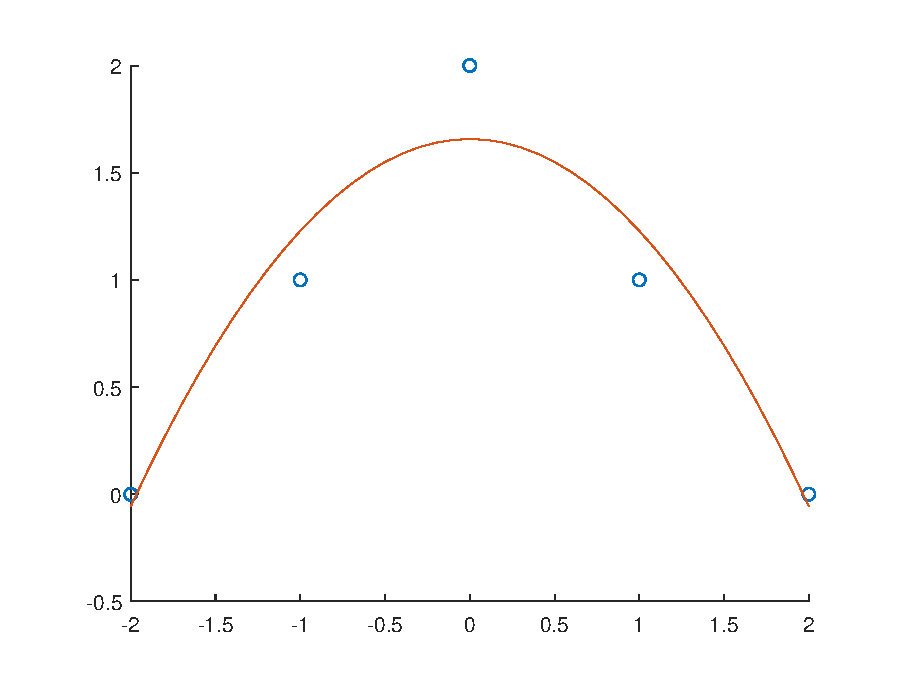
\includegraphics[scale=0.7]{e8_1.eps}
		\caption{第8章 第1题 二次多项式拟合结果}
	\end{figure}
	
	\textit{Code:}
	
% --------------------------代码--------------------------- %
\begin{lstlisting}[language = MATLAB]
% 第8章 第1题
x = [-2, -1, 0, 1, 2]; y = [0, 1, 2, 1, 0];
scatter(x, y); hold on;
x1 = sum(x);%sigma x
x2 = sum(x.^2);%sigma x^2
x3 = sum(x.^3);%sigma x^3
x4 = sum(x.^4);%sigma x^4
y1 = sum(y);%sigma y
x2y1 = sum(x.^2.*y);%sigma x^2 * y
x1y1 = sum(x.*y);%sigma x * y
de = ((5*x2-x1^2)*(5*x4-x2^2)-(5*x3-x2*x1)*(5*x3-x1*x2));
a = ((5*x2y1-x2*y1)*(5*x2-x1^2)-(5*x1y1-x1*y1)*(5*x3-x2*x1)) / de;
b = ((5*x1y1-x1*y1)*(5*x4-x2^2)-(5*x2y1-x2*y1)*(5*x3-x1*x2)) / de;
c = (y1-a*x2-b*x1) / 5;
plot(-2:0.1:2, a*(-2:0.1:2).^2+b*(-2:0.1:2)+c);
\end{lstlisting}

% ---------------------实验题目 2.---------------------- %
	\subsection{实验题目 2}
	\textit{Topic description:}
	
	研究发现单原子波函数的基本形式为$y=ae^{-bx}$,试根据实验室测试数据(如表所示)确定参数$a,b$。
	\begin{table}[htbp]
		\centering
		\begin{tabular}
			{c|cccc}
			\hline
			x&0&1&2&4 \\
			\hline
			y&2.010&1.210&0.740&0.450 \\
			\hline
		\end{tabular}
	\end{table}

	\textit{Answer:}
	
	\begin{figure}[htbp]
		\centering
		\includegraphics[scale=0.7]{e8_2.eps}
		\caption{第8章 第2题 拟合结果}
	\end{figure}
	
	指数曲线$y=ae^{-bx}$作为非线性拟合问题可简化为直线拟合问题
	\begin{equation*}
	\ln y=\ln a-bx
	\end{equation*}
	
	使用原数据$(x,y)$构造新数据$(\hat{x},\hat{y})$,其中$\hat{x}=x,\hat{y}=\ln y$,并去拟合曲线$\hat{y}=\alpha\hat{x}+\beta$,使用线性方程$y=a_1x+a_0$最小二乘拟合的参数求解公式
	\begin{equation*}
	\begin{split}
	a_0&=\frac{\sum\limits_{i=1}^{m}x_i^2\sum\limits_{i=1}^{m}y_i-\sum\limits_{i=1}^{m}x_iy_i\sum\limits_{i=1}^{m}x_i}{m\left(\sum\limits_{i=1}^{m}x_i^2\right)-\left(\sum\limits_{i=1}^{m}x_i\right)^2} \\
	a_1&=\frac{m\sum\limits_{i=1}^{m}x_iy_i-\sum\limits_{i=1}^{m}x_i\sum\limits_{i=1}^{m}y_i}{m\left(\sum\limits_{i=1}^{m}x_i^2\right)-\left(\sum\limits_{i=1}^{m}x_i\right)^2}
	\end{split}
	\end{equation*}
	
	求解出参数$\alpha,\beta$的值后根据$a=e^\beta,b=-\alpha$计算出参数$a,b$的值
	
	\textit{Code:}

% --------------------------------代码----------------------------------- %
\begin{lstlisting}[language = MATLAB]
% 第8章 第2题
x = [0, 1, 2, 4]; y = [2.010, 1.210, 0.740, 0.450];
scatter(x, y); hold on;
lny = log(y);
alpha = (4*sum(x.*lny)-sum(x)*sum(lny)) / (4*sum(x.^2)-sum(x)^2);
beta = (sum(x.^2)*sum(lny)-sum(x.*lny)*sum(x)) / (4*sum(x.^2)-sum(x)^2);
a = exp(beta); b=-alpha;
plot(0:0.1:4, a*exp(-b*(0:0.1:4)));
\end{lstlisting}
\newpage


\newpage
% --------------------------------第9章--------------------------------- %
	\section{Chapter 9\quad 特征值与特征向量}
	\label{sec:9}
	
% ------------------------实验题目 1.------------------------- %
	\subsection{实验题目 1}
	\textit{Topic description:}
	
	已知矩阵
	\[
	\begin{bmatrix}
	4&-1&1 \\
	-1&3&-2 \\
	1&-2&3
	\end{bmatrix}
	\]
	
	是一个对称矩阵,且其特征值为$\lambda_1=6,\lambda_2=3,\lambda_3=1$。
	
	分别利用幂法、对称幂法、反幂法求其最大特征值和特征向量
	
	注意:可取初始向量$\textbf{x}^{(0)}=(1\quad1\quad1)^T$。
	
	\textit{Answer:}
	
	\textbf{幂法:}
	
	假设$n\times n$矩阵$\mathbf{A}$有$n$个特征值$\lambda_1,\lambda_2,\dots,\lambda_n$与相应的线性无关的特征向量集$\{\mathbf{v}^{(1)},\mathbf{v}^{(2)},\mathbf{v}^{(3)},\dots,\mathbf{v}^{(n)}\}$。此外,假设$\mathbf{A}$恰有一个特征值$\lambda_1$的绝对值最大,使得$|\lambda_1|\geq|\lambda_2|\geq|\lambda_3|\geq\dots\geq|\lambda_n|\geq 0$。
	
	如果$\mathbf{x}$是$\mathbf{R}^n$上任意一个向量,$\{\mathbf{v}^{(1)},\mathbf{v}^{(2)},\mathbf{v}^{(3)},\dots,\mathbf{v}^{(n)}\}$是线性无关的说明存在常数$\beta_1,\beta_2,\dots,\beta_n$满足$$x=\sum_{j=1}^{n}\beta_j\mathbf{v}^{(j)}$$等式两边同时乘以$\mathbf{A},\mathbf{A}^2,\dots,\mathbf{A}^k$得出
	\begin{equation*}
	\begin{split}
	\mathbf{A}\mathbf{x}&=\sum_{j=1}^{n}\beta_j\mathbf{A}\mathbf{v}^{(j)}=\sum_{j=1}^{n}\beta_j\lambda_1\mathbf{v}^{(j)} \\
	\mathbf{A}^2\mathbf{x}&=\sum_{j=1}^{n}\beta_j\lambda_j\mathbf{A}\mathbf{v}^{(j)}=\sum_{j=1}^{n}\beta_j\lambda_1^2\mathbf{v}^{(j)} \\
	&\vdots \\
	\mathbf{A}^k\mathbf{x}&=\sum_{j=1}^{n}\beta_j\lambda_j^k\mathbf{v}^{(j)}
	\end{split}
	\end{equation*}将$\lambda_1^k$从最后一个方程的右边各项提取出来,那么$$\mathbf{A}^k\mathbf{x}=\lambda_1^k\sum_{j=1}^{n}\beta_j\left(\frac{\lambda_j}{\lambda_1}\right)\mathbf{v}^{(j)}$$因为对于所有$j=2,3,\dots,n$有$|\lambda_1|>|\lambda_j|$,则有$\lim\limits_{k\rightarrow\infty}(\lambda_j/\lambda_1)^k=0$,并且$$\lim\limits_{k\rightarrow\infty}\mathbf{A}^k\mathbf{x}=\lim\limits_{k\rightarrow\infty}\lambda_1^k\beta_1\mathbf{v}^{(1)}$$如果$|\lambda_1|<1$则该序列收敛于0,如果$|\lambda_1|>1$则该序列发散,前提条件是$\beta_1\neq 0$。
	
	通过以适当的方式调整$\mathbf{A}^k\mathbf{x}$的幂来保证方程的极限是有限的并且非零。调整过程为选择$\mathbf{x}$是与$||\cdot||_{\infty}$相关的单位向量$\mathbf{x}^{(0)}$并选择它的一个分量$x_{p_0}^{(0)}$满足
	\begin{equation*}
	x_{p_0}^{(0)}=1=||\mathbf{x}^{(0)}||_{\infty}
	\end{equation*}
	设$\mathbf{y}^{(1)}=\mathbf{A}\mathbf{x}^{(0)}$,并且定义$\mu^{(1)}=y_{p_0}^{(1)}$。那么
	\begin{equation*}
	\mu^{(1)}=y_{p_0}^{(1)}=\frac{y_{p_0}^{(1)}}{x_{p_0}^{(0)}}=\frac{\beta_1\lambda_1v_{p_0}^{(1)}+\sum\limits_{j=2}^{n}\beta_j\lambda_jv_{p_0}^{(j)}}{\beta_1v_{p_0}^{(1)}+\sum\limits_{j=2}^{n}\beta_jv_{p_0}^{(j)}}=\lambda_1\frac{\beta_1v_{p_0}^{(1)}+\sum\limits_{j=2}^{n}\beta_j(\lambda_j/\lambda_1)v_{p_0}^{(1)}}{\beta_1v_{p_0}^{(1)}+\sum\limits_{j=2}^{n}\beta_jv_{p_0}^{(1)}}
	\end{equation*}
	设$p_1$是满足
	\begin{equation*}
	|y_{p_1}^{(1)}|=||\mathbf{y}^{(1)}||_\infty
	\end{equation*}
	的最小整数,定义
	\begin{equation*}
	\mathbf{x}^{(1)}=\frac{1}{y_{p_1}^{(1)}}\mathbf{y}^{(1)}=\frac{1}{y_{p_1}^{(1)}}\mathbf{A}\mathbf{x}^{(0)}
	\end{equation*}
	则
	\begin{equation*}
	x_{p_1}^{(1)}=1=||\mathbf{x}^{(1)}||_\infty
	\end{equation*}
	现定义
	\begin{equation*}
	\mathbf{y}^{(2)}=\mathbf{Ax}^{(1)}=\frac{1}{y_{p_1}^{(1)}}\mathbf{A}^{2}\mathbf{x}^{(0)}
	\end{equation*}
	和
	\begin{equation*}
	\mu^{(2)}=y_{p_1}^{(2)}=\frac{y_{p_1}^{(2)}}{x_{p_1}^{(1)}}=\frac{[\beta_1\lambda_1^2v_{p_1}^{(1)}+\sum\limits_{j=2}^{n}\beta_j\lambda_j^2v_{p_1}^{(j)}]/y_{p_1}^{(1)}}{[\beta_1\lambda_1v_{p_1}^{(1)}+\sum\limits_{j=2}^{n}\beta_j\lambda_jv_{p_1}^{(j)}]/y_{p_1}^{(1)}}=\lambda_1\frac{\beta_1v_{p_1}^{(1)}+\sum\limits_{j=2}^{n}\beta_j(\lambda_j/\lambda_1)^2v_{p_1}^{(j)}}{\beta_1v_{p_1}^{(1)}+\sum\limits_{j=2}^{n}\beta_j(\lambda_j/\lambda_1)v_{p_1}^{(j)}}
	\end{equation*}
	设$p_2$是满足
	\begin{equation*}
	|y_{p_2}^{(2)}|=||\mathbf{y}^{(2)}||_\infty
	\end{equation*}
	的最小整数,并且定义
	\begin{equation*}
	\mathbf{x}^{(2)}=\frac{1}{y_{p_2}^{(2)}}\mathbf{y}^{(2)}=\frac{1}{y_{p_2}^{(2)}}\mathbf{A}\mathbf{x}^{(1)}=\frac{1}{y_{p_2}^{(2)}y_{p_1}^{(1)}}\mathbf{A}^2\mathbf{x}^{(0)}
	\end{equation*}
	由类似方法,定义向量序列$\{\mathbf{x}^{(m)}\}_{m=0}^\infty$和$\{\mathbf{y}^{(m)}\}_{m=0}^\infty$以及由$\mathbf{y}^{(m)}=\mathbf{A}\mathbf{x}^{(m-1)}$归纳定义的比例因子序列$\{\mu^{(m)}\}_{m=0}^\infty$
	\begin{equation*}
	\mu^{(m)}=y_{p_{m-1}}^{(m)}=\lambda_1\frac{\beta_1v_{p_{m-1}}^{(1)}+\sum\limits_{j=2}^{n}\beta_j(\lambda_j/\lambda_1)^mv_{p_{m-1}}^{(j)}}{\beta_1v_{p_{m-1}}^{(1)}+\sum\limits_{j=2}^{n}\beta_j(\lambda_j/\lambda_1)^{m-1}v_{p_{m-1}}^{(j)}}
	\end{equation*}
	和
	\begin{equation*}
	\mathbf{x}^{(m)}=\frac{\mathbf{y}^{(m)}}{y_{p_m}^{(m)}}=\frac{\mathbf{A}^{m}\mathbf{x}^{(0)}}{\prod\limits_{k=1}^my_{p_k}^{(k)}}
	\end{equation*}
	这里每一步中$p_m$用雷表示满足
	\begin{equation*}
	|y_{p_m}^m|=||\mathbf{y}^{(m)}||_\infty
	\end{equation*}
	的最小整数。
	
	因为对$j=2,3,\dots,n$由$|\lambda_j/\lambda_1|<1$,只要选择$\mathbf{x}^{(0)}$满足$\beta_1\neq 0$,就有$\lim\limits_{m\rightarrow\infty}\mu^{(m)}=\lambda_1$。而且,向量序列$\{\mathbf{x}^{(m)}\}_{m=0}^\infty$收敛于与$\lambda_1$相关的其$l_\infty$范数为$1$的特征向量。
	
	\textbf{对称幂法:}
	
	假设$A$是对称矩阵,$A$由$n$个实数特征向量$|\lambda_1|>|\lambda_2|>\dots>|\lambda_n|$,对应$n$个标准正交的特征向量$\{\mathbf{v}^{(1)},\mathbf{v}^{(2)},\dots,\mathbf{v}^{(n)}\}$
	
	$\forall x_0\in R^n,x_0=\beta_1\mathbf{v}^{(1)}+\beta_2\mathbf{v}^{(2)}+\dots+\beta_n\mathbf{v}^{(n)}$
	
	对于$x_k=A^kx_0,x_k=\beta_1\lambda_1^kv^{(1)}+\beta_2\lambda_2^kv^{(2)}+\dots+\beta_n\lambda_nv^{(n)}$
	
	因为n个特征向量标准正交,因此
	\begin{equation*}
		x_k^Tx_k=\sum_{j=1}^{n}\beta_j^2\lambda_j^{2k}=\beta_1^2\lambda_1^{2k}[1+\sum_{j=2}^{n}\left(\frac{\beta_j}{\beta_1}\right)^2\left(\frac{\lambda_j}{\lambda_1}\right)^{2k}]
	\end{equation*}且
	\begin{equation*}
	x_k^TAx_k=\sum_{j=1}^{n}\beta_j^2\lambda_j^{2k+1}=\beta_1^2\lambda_1^{2k+1}[1+\sum_{j=2}^{n}\left(\frac{\beta_j}{\beta_1}\right)^2\left(\frac{\lambda_j}{\lambda_1}\right)^{2k+1}]
	\end{equation*}因此
	\begin{equation*}
	\begin{split}
	\lim\limits_{k\rightarrow\infty}\frac{x_k^TAx_k}{x_k^Tx_k}&=\lambda_1\\
	\lim\limits_{k\rightarrow\infty}\frac{x_k}{||x_k||_2}&=\frac{v^{(1)}}{||v^{(1)}||_2}
	\end{split}
	\end{equation*}
	
	\textbf{反幂法:}
	
	反幂法是对幂法的修改,可就给出更快的收敛性。它用来确定与特定数$q$最接近的$A$的特征值。设A为$n\times n$非奇异矩阵,$\lambda$和$v$为对应的特征向量,即$Au=\lambda v$。由于$(A-qI)^{-1}v=\frac{1}{\lambda-q}v$。对$(A-qI)^{-1}$应用幂法,得出
	\begin{equation*}
	y^{(m)}=(A-qI)^{-1}x(m-1)
	\end{equation*}
	令
	\begin{equation*}
	\mu^{(m)}=y_{p_{m-1}}^{(m)}=\frac{y_{p_m-1}{(m)}}{x_{p_m-1}{(m-1)}}=\frac{\sum\limits_{j=1}^{n}\beta_j\frac{1}{(\lambda_j-q)^m}v_{p_{m-1}}^{(j)}}{\sum\limits_{j=1}^{n}\beta_j\frac{1}{(\lambda_j-q)^{m-1}}v_{p_{m-1}}^{(j)}}
	\end{equation*}
	令$p_m$表示
	\begin{equation*}
	|y_{p_m}^{(m)}|=||y^{(m)}||_\infty
	\end{equation*}
	的最小整数,序列$\{\mu^{(m)}\}$收敛于
	\begin{equation*}
	\frac{1}{|\lambda_k-q|}=\max\limits_{1\leq j\leq n}\frac{1}{|\lambda_i-q|}
	\end{equation*}
	
	$y^{(m)}$可通过方程
	\begin{equation*}
	(A-qI)y^{(m)}=x^{(m-1)}
	\end{equation*}得到。
	
	\begin{table}[htbp]
		\centering
		\caption{第9章 第1题 不同方法求对称矩阵的最大特征值与特征向量}\label{e9_1}
		\begin{tabular}
			{c|c|c|c}
			\hline
			&迭代次数&最大特征值&特征向量 \\
			\hline
			幂法&18&6&$[1,-1,1]$ \\
			\hline
			对称幂法&17&6&$[1,-1,1]$ \\
			\hline
			反幂法&14&6&$[1,-1,1]$ \\
			\hline
		\end{tabular}
	\end{table}
	
	\begin{figure}[htbp]
		\centering
		\subfigure[$(1\quad1\quad1)^T$]{
			\includegraphics[scale=0.59]{e9_1_4.eps}
		} \quad
		\subfigure[$(1\quad0.1\quad0.2)^T$]{
			\includegraphics[scale=0.59]{e9_1_5.eps}
		} \quad
		\subfigure[$(1\quad1\quad2)^T$]{
			\includegraphics[scale=0.59]{e9_1_6.eps}
		} \quad
		\subfigure[$(1\quad-0.1\quad0.2)^T$]{
			\includegraphics[scale=0.59]{e9_1_7.eps}
		}
		\caption{第9章 第1题 不好的初始向量导致的迭代过程}\label{e9_1_1}
	\end{figure}
	
	通过表(\ref{e9_1})可以发现三种方法都求得了最大的特征值及对应的特征向量,但是迭代次数不同。
	
	反幂法本身是对幂法的改近,可以更快地收敛,实验结果里反幂法用的迭代次数比幂法和对称幂法要少,收敛速率最快。
	
	但是反幂法要求好的初始向量的选取,如果初始向量不够好,就会如图(\ref{e9_1_1})里所示的,在给定的迭代次数里找不到正确的解(a),或者可能初始向量的选取导致一开始与其他特征值比较接近,因此很快虽然迭代的如预期的那样很快,但却收敛到了其他的特征值(bc),又或者阴差阳错地虽然可以收敛到正确的最大特征值,但收敛次数远超其他方法(d)。
	
	实验中反幂法使用给定的初始向量$\textbf{x}^{(0)}=(1\quad1\quad1)^T$效果不好,因此随机尝试了一些初始向量,在使用$\textbf{x}^{(0)}=(1\quad-1\quad2)^T$时得到了表中结果。
	
	\begin{figure}[htbp]
		\centering
		\subfigure[幂法]{
			\includegraphics[scale=0.6]{e9_1_1.eps}
		} \quad
		\subfigure[对称幂法]{
			\includegraphics[scale=0.6]{e9_1_2.eps}
		} \quad
		\subfigure[反幂法]{
			\includegraphics[scale=0.6]{e9_1_3.eps}
		}
		\caption{第9章 第1题 不同方法求对称矩阵的最大特征值与特征向量}\label{e9_1_2}
	\end{figure}

	\textit{algorithm:}
	
	\begin{algorithm}
		\caption{the Power Method}
		\KwIn{dimension $n$; matrix $\mathbf{A}$; vector $\mathbf{x}$; tolerance $TOL$; maximum number of iterations $N$;}
		\KwOut{approximate eigenvalue $\mu$; approximate eigenvector $\mathbf{x}$(with $||\mathbf{x}||_\infty=1$) or a message that the number of iterations was exceeded.}
		Set $k=1;$
		
		Find the smallest integer $p$ with $1\leq p\leq n$ and $|x_p|=||\mathbf{x}||_\infty$;
		
		Set $\mathbf{x}=\mathbf{x}/x_p;$
		
		\While{$k\leq N$}
		{
			Set $\mathbf{y=Ax}; \mu=y_p;$
			
			Find the smallest integer $p$ with $1\leq p\leq n$ and $|y_p|=||\mathbf{y}||_\infty$;
			
			\If{$y_p=0$}
			{
				OUTPUT($x$);
				
				OUTPUT('A has the eigenvalue 0, select a new vector $\mathbf{x}$ and restart');
				
				STOP;
			}
			
			Set $ERR=||\mathbf{x}-(\mathbf{y}/y_p)||_\infty; \mathbf{x}=\mathbf{y}/y_p;$
			
			\If{$ERR<TOL$}
			{
				OUTPUT($\mu,\mathbf{x}$);(Procedure completed successfully)
				
				STOP;
			}
		
			Set $k=k+1$;
		}
		
		OUTPUT('Maximum number of iterations exceeded');(Procedure completed unsuccessfully)
		
		STOP;
	\end{algorithm}

	\begin{algorithm}
		\caption{Symmetric Power Method}
		\KwIn{dimension $n$; matrix $\mathbf{A}$; vector $\mathbf{x}$; tolerance $TOL$; maximum number of iterations $N$;}
		\KwOut{approximate eigenvalue $\mu$; approximate eigenvector $\mathbf{x}$(with $||\mathbf{x}||_2=1$) or a message that the number of iterations was exceeded.}
		Set $k=1; \mathbf{x}=\mathbf{x}/||\mathbf{x}||_2;$
		
		\While{$k\leq N$}
		{
			Set $\mathbf{y=Ax}; \mu=\mathbf{x^Ty};$
			
			\If{$||y||_2=0$}
			{
				OUTPUT($x$);
				
				OUTPUT('A has the eigenvalue 0, select a new vector $\mathbf{x}$ and restart');
				
				STOP;
			}
			
			Set $ERR=||\mathbf{x}-\mathbf{y}/||\mathbf{y}||_2||_2; \mathbf{x}=\mathbf{y}/||\mathbf{y}||_2;$
			
			\If{$ERR<TOL$}
			{
				OUTPUT($\mu,\mathbf{x}$);(Procedure completed successfully)
				
				STOP;
			}
			
			Set $k=k+1$;
		}
		
		OUTPUT('Maximum number of iterations exceeded');(Procedure completed unsuccessfully)
		
		STOP;
	\end{algorithm}

	\begin{algorithm}
		\caption{the Inverse Power Method}
		\KwIn{dimension $n$; matrix $\mathbf{A}$; vector $\mathbf{x}$; tolerance $TOL$; maximum number of iterations $N$;}
		\KwOut{approximate eigenvalue $\mu$; approximate eigenvector $\mathbf{x}$(with $||\mathbf{x}||_\infty=1$) or a message that the number of iterations was exceeded.}
		Set $q=\frac{\mathbf{x^TAx}}{\mathbf{x^Tx}}$
		
		Set $k=1;$
		
		Find the smallest integer $p$ with $1\leq p\leq n$ and $|x_p|=||\mathbf{x}||_\infty$;
		
		Set $\mathbf{x}=\mathbf{x}/x_p;$
		
		\While{$k\leq N$}
		{
			Set the linear system $(\mathbf{A}-q\mathbf{I})\mathbf{y}=\mathbf{x}$;
			
			If the system doesn't have a unique solution, then OUTPUT('q is an eigenvalue', $q$);
			
			Set $\mu=y_p;$
			
			Find the smallest integer $p$ with $1\leq p\leq n$ and $|y_p|=||\mathbf{y}||_\infty$;
			
			Set $ERR=||\mathbf{x}-(\mathbf{y}/y_p)||_\infty; \mathbf{x}=\mathbf{y}/y_p;$
			
			\If{$ERR<TOL$}
			{
				Set $\mu=(1/\mu)+q;$
				
				OUTPUT($\mu,\mathbf{x}$);(Procedure completed successfully)
				
				STOP;
			}
			
			Set $k=k+1$;
		}
		
		OUTPUT('Maximum number of iterations exceeded');(Procedure completed unsuccessfully)
		
		STOP;
	\end{algorithm}

	\textit{Code:}
	
% ---------------------代码----------------------- %
\begin{lstlisting}[language = MATLAB]
function [mu,x,k] = PowerMethod(n,A,x,tol,N)
% 幂法
	pre_x = x;
	mu = zeros(N, 1);
	k = 1;
	[v, p] = max(abs(x));
	x = x ./ x(p);
	while k <= N
		y = A * x;
		mu(k) = y(p);
		[v, p] = max(abs(y));
		if v == 0
			disp('Eigenvector'); disp(pre_x);
			disp('A has the eigenvalue 0,select a new vector x and restart');
			return;  % STOP
		end
		err = max(abs(x - y ./ y(p)));
		x = y ./ y(p);
		if err < tol
			plot(1:k, mu(1:k));
			mu = mu(k);
		return;  % STOP
		end
		k = k + 1;
	end
	if k > N
		disp('Maximum number of iterations exceeded.Procedure PowerMethod completed unsuccessfully');
	end
end
\end{lstlisting}

\begin{lstlisting}[language = MATLAB]
function [mu,x,k] = SymmetricPowerMethod(n,A,x,tol,N)
% 对称幂法
	mu = zeros(N, 1);
	k = 1;
	x = x / norm(x);
	while k <= N
		y = A * x;
		mu(k) = x' * y;
		if norm(y) == 0
			disp('Eigenvector'); disp(pre_x);
			disp('A has the eigenvalue 0,select a new vector x and restart');
			return;  % STOP
		end
		err = norm(x - y / norm(y));
		x = y / norm(y);
		if err < tol
			plot(1:k, mu(1:k));
			mu = mu(k);
			x = x / max(abs(x));
		return;  % STOP
		end
		k = k + 1;
	end
	if k > N
		disp('Maximum number of iterations exceeded.Procedure SymmetricPowerMethod completed unsuccessfully');
	end
end
\end{lstlisting}

\begin{lstlisting}[language = MATLAB]
function [mu,x,k] = InversePowerMethod(n,A,x,tol,N)
% 反幂法
	mu = zeros(N, 1);
	q = (x' * A * x) / (x' * x);
	k = 1;
	[v, p] = max(abs(x));
	x = x ./ x(p);
	while k <= N
		[L, U, y] = LUDecomposition(n, A - q * eye(n), x);
		mu(k) = y(p);
		[v, p] = max(abs(y));
		err = max(abs(x - y ./ y(p)));
		x = y ./ y(p);
		if err < tol
			plot(1:k, 1 ./ mu(1:k) + q);
			mu = 1 / mu(k) + q;
			return;  % STOP
		end
		k = k + 1;
	end
	if k > N
		plot(1:N, 1 ./ mu(1:N) + q);
		k = N; mu = 1 / mu(N) + q;
		disp(err)
		disp('Maximum number of iterations exceeded.Procedure InversePowerMethod completed unsuccessfully');
	end
end
\end{lstlisting}
	使用上面3种方法分别计算
\begin{lstlisting}[language = MATLAB]
% 第9章 第1题
A = [4, -1, 1;
	-1, 3, -2;
	1, -2, 3];
x = [1, -1, 2]'; n = 3; tol = 1e-9; N = 100000;
[mu1, x1, k1] = PowerMethod(n, A, x, tol, N);
[mu2, x2, k2] = SymmetricPowerMethod(n, A, x, tol, N);
[mu3, x3, k3] = InversePowerMethod(n, A, x, tol, N);
\end{lstlisting}
	
% ----------------------------实验题目 2.-------------------------------- %
	\subsection{实验题目 2}
	\textit{Topic description:}
	
	分别利用Householder变换和Givens旋转变化方法求A的QR分解
	\[
	A=\begin{bmatrix}
	1&0&0 \\
	1&1&0 \\
	1&1&1 \\
	1&1&1
	\end{bmatrix}
	\]
	
	写出每一步具体求解过程,及最终分解结果
	
	\textit{Answer:}
	
	\textbf{Householder}:
	
	\begin{equation*}
	\begin{aligned}
	H_1=\begin{bmatrix}
	-0.5&-0.5&-0.5&-0.5 \\
	-0.5&0.8333&-1.667&-1.667 \\
	-0.5&-1.667&0.8333&-1.667 \\
	-0.5&-1.667&-1.667&0.8333
	\end{bmatrix}&\quad\Rightarrow\quad
	&H_1A=\begin{bmatrix}
	-2&-1.5&-1 \\
	0&0.5&-0.3333 \\
	0&0.5&0.6667 \\
	0&0.5&0.6667
	\end{bmatrix} \\
	H_2=\begin{bmatrix}
	1&0&0&0 \\
	0&-0.5774&-0.5774&-0.5774 \\
	0&-0.5774&0.7887&-0.2113 \\
	0&-0.5774&-0.2113&0.7887
	\end{bmatrix}&\quad\Rightarrow\quad
	&H_2H_1A=\begin{bmatrix}
	-2&-1.5&-1 \\
	0&-0.866&-0.5774 \\
	0&0&0.5774 \\
	0&0&0.5774
	\end{bmatrix} \\
	H_3=\begin{bmatrix}
	1&0&0&0 \\
	0&1&0&0 \\
	0&0&-0.7071&-0.7071 \\
	0&0&-0.7071&0.7071
	\end{bmatrix}&\quad\Rightarrow\quad
	&H_3H_2H_1A=\begin{bmatrix}
	-2&-1.5&-1 \\
	0&-0.866&-0.5774 \\
	0&0&-0.8165 \\
	0&0&0
	\end{bmatrix}
	\end{aligned}
	\end{equation*}
	
	最后求出的QR矩阵为:
	\[
	Q=\begin{bmatrix}
	-0.5&0.866&0&0 \\
	-0.5&-0.2887&0.8165&0 \\
	-0.5&-0.2887&-0.4082&-0.7071 \\
	-0.5&-0.2887&-0.4082&0.7071
	\end{bmatrix}\quad
	R=\begin{bmatrix}
	-2&-1.5&-1 \\
	0&-0.866&-0.5774 \\
	0&0&-0.8165
	\end{bmatrix}
	\]
	
	\textbf{Givens}:
	
	\begin{equation*}
	\begin{aligned}
	G_1=\begin{bmatrix}
	0.7071&0&0&0.7071 \\
	0&1&0&0 \\
	0&0&1&0 \\
	-0.7071&0&0&0.7071
	\end{bmatrix} &\quad\Rightarrow\quad
	&G_1A=\begin{bmatrix}
	1.4142&0.7071&0.7071 \\
	1&1&0 \\
	1&1&1 \\
	0&0.7071&0.7071
	\end{bmatrix} \\
	G_2=\begin{bmatrix}
	0.8165&0&0.5774&0 \\
	0&1&0&0 \\
	-0.5774&0&0.8165&0 \\
	0&0&0&1
	\end{bmatrix} &\quad\Rightarrow\quad
	&G_2G_1A=\begin{bmatrix}
	1.7321&1.1547&1.1547 \\
	1&1&0 \\
	0&0.4082&0.4082 \\
	0&0.7071&0.7071
	\end{bmatrix} \\
	G_3=\begin{bmatrix}
	0.866&0.5&0&0 \\
	-0.5&0.866&0&0 \\
	0&0&1&0 \\
	0&0&0&1
	\end{bmatrix} &\quad\Rightarrow\quad
	&G_3G_2G_1A=\begin{bmatrix}
	2&1.5&1 \\
	0&0.2887&-0.5774 \\
	0&0.4082&0.4082 \\
	0&0.7071&0.7071
	\end{bmatrix} \\
	G_4=\begin{bmatrix}
	1&0&0&0 \\
	0&0.378&0&0.9258 \\
	0&0&1&0 \\
	0&-0.9258&0&0.3780
	\end{bmatrix} &\quad\Rightarrow\quad
	&G_4G_3G_2G_1A=\begin{bmatrix}
	2&1.5&1 \\
	0&0.7638&0.4364 \\
	0&0.4082&0.4082 \\
	0&0&0.8018
	\end{bmatrix} \\
	G_5=\begin{bmatrix}
	1&0&0&0 \\
	0&0.8819&0.4714&0 \\
	0&-0.4714&0.8819&0 \\
	0&0&0&1
	\end{bmatrix} &\quad\Rightarrow\quad
	&G_5G_4G_3G_2G_1A=\begin{bmatrix}
	2&1.5&1 \\
	0&0.866&0.5774 \\
	0&0&0.1543 \\
	0&0&0.8018
	\end{bmatrix} \\
	G_6=\begin{bmatrix}
	1&0&0&0 \\
	0&1&0&0 \\
	0&0&0.189&0.982 \\
	0&0&-0.982&0.189
	\end{bmatrix} &\quad\Rightarrow\quad
	&G_6G_5G_4G_3G_2G_1A=\begin{bmatrix}
	2&1.5&1 \\
	0&0.866&0.5774 \\
	0&0&0.8165 \\
	0&0&0
	\end{bmatrix}
	\end{aligned}
	\end{equation*}
	
	最后求出的QR矩阵为:
	\[
	Q=\begin{bmatrix}
		0.5&-0.866&0&0 \\
		0.5&0.2887&-0.8165&0 \\
		0.5&0.2887&0.4082&-0.7071 \\
		0.5&0.2887&0.4082&0.7071
	\end{bmatrix} \quad
	R=\begin{bmatrix}
		2&1.5&1 \\
		0&0.866&0.5774 \\
		0&0&0.8165
	\end{bmatrix}
	\]
	
	\textit{Code:}
	
% --------------------------------代码----------------------------------- %
\begin{lstlisting}[language = MATLAB]
function [H,R,b] = HouseHolder(n,A,b)
% HouseHolder变换
	I = eye(n);
	H = eye(n);
	for i = 1 : size(A, 2)
		a = [zeros(i-1, 1);A(i:size(A,1), i)];
		alpha = -sign(a(i)) * norm(a);
		e = zeros(n, 1); e(i) = 1;
		v = a - alpha * e;
		disp(['v', num2str(i)]); disp(v);
		h = I - 2 * (v * v') / (v' * v);
		H = h * H;
		disp(['H', num2str(i)]); disp(h);
		A = h * A;
		b = h * b;
		disp(['A', num2str(i)]); disp(A);
	end
	R = A(1:size(A, 2),1:size(A, 2));
end
\end{lstlisting}

\begin{lstlisting}[language = MATLAB]
function [G,R,b] = Givens(n,A,b)
% Givens变换
	G = eye(n);
	for col = 1 : size(A, 2)  % 从第1列到最后1列
		for row = size(A, 1) : -1 : col + 1  % 从最后1行到第1行
			if A(row, col) == 0
				continue;
			end
			disp([num2str(row), ' ', num2str(col)]);
			c = A(col, col) / sqrt(A(col, col)^2+A(row, col)^2);
			s = A(row, col) / sqrt(A(col, col)^2+A(row, col)^2);
			g = eye(size(A, 1));
			g(col, col) = c; g(row, col) = -s; g(col, row) = s; g(row, row) = c;
			disp('G'); disp(g);
			G = g * G;
			A = g * A;
			disp('A'); disp(A);
			b = g * b;
		end
	end
	R = A(1:size(A, 2),1:size(A, 2));
end
\end{lstlisting}

\begin{lstlisting}[language = MATLAB]
A = [1, 0, 0;
	1, 1, 0;
	1, 1, 1;
	1, 1, 1];
b = [1;0;1;0];
[H, R, b] = HouseHolder(size(A, 1), A, b);
[G, R, b] = Givens(size(A, 1), A, b);
\end{lstlisting}
\newpage


\end{document}